% Options for packages loaded elsewhere
\PassOptionsToPackage{unicode}{hyperref}
\PassOptionsToPackage{hyphens}{url}
%
\documentclass[
]{article}
\usepackage{amsmath,amssymb}
\usepackage{iftex}
\ifPDFTeX
  \usepackage[T1]{fontenc}
  \usepackage[utf8]{inputenc}
  \usepackage{textcomp} % provide euro and other symbols
\else % if luatex or xetex
  \usepackage{unicode-math} % this also loads fontspec
  \defaultfontfeatures{Scale=MatchLowercase}
  \defaultfontfeatures[\rmfamily]{Ligatures=TeX,Scale=1}
\fi
\usepackage{lmodern}
\ifPDFTeX\else
  % xetex/luatex font selection
\fi
% Use upquote if available, for straight quotes in verbatim environments
\IfFileExists{upquote.sty}{\usepackage{upquote}}{}
\IfFileExists{microtype.sty}{% use microtype if available
  \usepackage[]{microtype}
  \UseMicrotypeSet[protrusion]{basicmath} % disable protrusion for tt fonts
}{}
\makeatletter
\@ifundefined{KOMAClassName}{% if non-KOMA class
  \IfFileExists{parskip.sty}{%
    \usepackage{parskip}
  }{% else
    \setlength{\parindent}{0pt}
    \setlength{\parskip}{6pt plus 2pt minus 1pt}}
}{% if KOMA class
  \KOMAoptions{parskip=half}}
\makeatother
\usepackage{xcolor}
\usepackage[margin=1in]{geometry}
\usepackage{color}
\usepackage{fancyvrb}
\newcommand{\VerbBar}{|}
\newcommand{\VERB}{\Verb[commandchars=\\\{\}]}
\DefineVerbatimEnvironment{Highlighting}{Verbatim}{commandchars=\\\{\}}
% Add ',fontsize=\small' for more characters per line
\usepackage{framed}
\definecolor{shadecolor}{RGB}{248,248,248}
\newenvironment{Shaded}{\begin{snugshade}}{\end{snugshade}}
\newcommand{\AlertTok}[1]{\textcolor[rgb]{0.94,0.16,0.16}{#1}}
\newcommand{\AnnotationTok}[1]{\textcolor[rgb]{0.56,0.35,0.01}{\textbf{\textit{#1}}}}
\newcommand{\AttributeTok}[1]{\textcolor[rgb]{0.13,0.29,0.53}{#1}}
\newcommand{\BaseNTok}[1]{\textcolor[rgb]{0.00,0.00,0.81}{#1}}
\newcommand{\BuiltInTok}[1]{#1}
\newcommand{\CharTok}[1]{\textcolor[rgb]{0.31,0.60,0.02}{#1}}
\newcommand{\CommentTok}[1]{\textcolor[rgb]{0.56,0.35,0.01}{\textit{#1}}}
\newcommand{\CommentVarTok}[1]{\textcolor[rgb]{0.56,0.35,0.01}{\textbf{\textit{#1}}}}
\newcommand{\ConstantTok}[1]{\textcolor[rgb]{0.56,0.35,0.01}{#1}}
\newcommand{\ControlFlowTok}[1]{\textcolor[rgb]{0.13,0.29,0.53}{\textbf{#1}}}
\newcommand{\DataTypeTok}[1]{\textcolor[rgb]{0.13,0.29,0.53}{#1}}
\newcommand{\DecValTok}[1]{\textcolor[rgb]{0.00,0.00,0.81}{#1}}
\newcommand{\DocumentationTok}[1]{\textcolor[rgb]{0.56,0.35,0.01}{\textbf{\textit{#1}}}}
\newcommand{\ErrorTok}[1]{\textcolor[rgb]{0.64,0.00,0.00}{\textbf{#1}}}
\newcommand{\ExtensionTok}[1]{#1}
\newcommand{\FloatTok}[1]{\textcolor[rgb]{0.00,0.00,0.81}{#1}}
\newcommand{\FunctionTok}[1]{\textcolor[rgb]{0.13,0.29,0.53}{\textbf{#1}}}
\newcommand{\ImportTok}[1]{#1}
\newcommand{\InformationTok}[1]{\textcolor[rgb]{0.56,0.35,0.01}{\textbf{\textit{#1}}}}
\newcommand{\KeywordTok}[1]{\textcolor[rgb]{0.13,0.29,0.53}{\textbf{#1}}}
\newcommand{\NormalTok}[1]{#1}
\newcommand{\OperatorTok}[1]{\textcolor[rgb]{0.81,0.36,0.00}{\textbf{#1}}}
\newcommand{\OtherTok}[1]{\textcolor[rgb]{0.56,0.35,0.01}{#1}}
\newcommand{\PreprocessorTok}[1]{\textcolor[rgb]{0.56,0.35,0.01}{\textit{#1}}}
\newcommand{\RegionMarkerTok}[1]{#1}
\newcommand{\SpecialCharTok}[1]{\textcolor[rgb]{0.81,0.36,0.00}{\textbf{#1}}}
\newcommand{\SpecialStringTok}[1]{\textcolor[rgb]{0.31,0.60,0.02}{#1}}
\newcommand{\StringTok}[1]{\textcolor[rgb]{0.31,0.60,0.02}{#1}}
\newcommand{\VariableTok}[1]{\textcolor[rgb]{0.00,0.00,0.00}{#1}}
\newcommand{\VerbatimStringTok}[1]{\textcolor[rgb]{0.31,0.60,0.02}{#1}}
\newcommand{\WarningTok}[1]{\textcolor[rgb]{0.56,0.35,0.01}{\textbf{\textit{#1}}}}
\usepackage{longtable,booktabs,array}
\usepackage{calc} % for calculating minipage widths
% Correct order of tables after \paragraph or \subparagraph
\usepackage{etoolbox}
\makeatletter
\patchcmd\longtable{\par}{\if@noskipsec\mbox{}\fi\par}{}{}
\makeatother
% Allow footnotes in longtable head/foot
\IfFileExists{footnotehyper.sty}{\usepackage{footnotehyper}}{\usepackage{footnote}}
\makesavenoteenv{longtable}
\usepackage{graphicx}
\makeatletter
\def\maxwidth{\ifdim\Gin@nat@width>\linewidth\linewidth\else\Gin@nat@width\fi}
\def\maxheight{\ifdim\Gin@nat@height>\textheight\textheight\else\Gin@nat@height\fi}
\makeatother
% Scale images if necessary, so that they will not overflow the page
% margins by default, and it is still possible to overwrite the defaults
% using explicit options in \includegraphics[width, height, ...]{}
\setkeys{Gin}{width=\maxwidth,height=\maxheight,keepaspectratio}
% Set default figure placement to htbp
\makeatletter
\def\fps@figure{htbp}
\makeatother
\setlength{\emergencystretch}{3em} % prevent overfull lines
\providecommand{\tightlist}{%
  \setlength{\itemsep}{0pt}\setlength{\parskip}{0pt}}
\setcounter{secnumdepth}{-\maxdimen} % remove section numbering
\ifLuaTeX
  \usepackage{selnolig}  % disable illegal ligatures
\fi
\IfFileExists{bookmark.sty}{\usepackage{bookmark}}{\usepackage{hyperref}}
\IfFileExists{xurl.sty}{\usepackage{xurl}}{} % add URL line breaks if available
\urlstyle{same}
\hypersetup{
  pdftitle={RAZONES DEL VOTO VALENCIANISTA EN LAS ELECCIONES AUTONÓMICAS DEL 2023},
  pdfauthor={Tomàs Ferrandis Moscardó},
  hidelinks,
  pdfcreator={LaTeX via pandoc}}

\title{RAZONES DEL VOTO VALENCIANISTA EN LAS ELECCIONES AUTONÓMICAS DEL
2023}
\author{Tomàs Ferrandis Moscardó}
\date{2024-01-29}

\begin{document}
\maketitle

{
\setcounter{tocdepth}{2}
\tableofcontents
}
\hypertarget{resumen}{%
\section{1.RESUMEN}\label{resumen}}

El presente trabajo de investigación estudia porqué el voto a
formaciones políticas valencianistas en las Elecciones Autonómicas del
2023 se dio de forma desigual en las diferentes comarcas valencianas. El
estudio se centrará en posibles causas como el idioma predominante, el
carácter periférico o la ruralidad de la comarca.

\hypertarget{abstract}{%
\subsection{Abstract}\label{abstract}}

This research study studies why the vote for Valencian political
formations in the 2023 autonumous elections of the Valencian Community
occurred unequally in the different Valencian regions (comarcas). The
study will focus on possible causes such as the predominant language,
the peripheral nature or the rurality of the region.

\hypertarget{palabras-clave}{%
\section{2.PALABRAS CLAVE}\label{palabras-clave}}

Voto valencianista, elecciones autonómicas valencianas 2023, comarca,
ruralidad, centralidad, periferia, provincialismo, valencianohablante,
castellanohablante.

\hypertarget{justificaciuxf3n-de-la-relevancia-de-la-investigaciuxf3n}{%
\section{3.JUSTIFICACIÓN DE LA RELEVANCIA DE LA
INVESTIGACIÓN}\label{justificaciuxf3n-de-la-relevancia-de-la-investigaciuxf3n}}

La presente investigación se centrará en averiguar las razones del voto
desigual en las elecciones autonómicas del 2023 a lo largo del mapa
comarcal de la Comunidad Valenciana de las fuerzas políticas
estrictamente valencianas cuyo discurso o programa responde
fundamentalmente al clivaje identitario. Es decir, aquellos partidos que
nacen del ``conflicto entre la cultura central que constituye la nación
y la resistencia creciente de las poblaciones sometidas de las
provincias y las periferias, étnicas, lingüísticas o religiosamente
diferenciadas'' (Lipset y Rokkan). No se pretende diferenciar entre
opciones más nacionalistas o más regionalistas ni tampoco entrar en
otras consideraciones referentes a otros clivajes que no sea
estrictamente el que atañe al debate ``centro-periferia''\footnote{No
  debe confundirse con el clivaje ``centro-periferia'' definitorio de un
  partido nacionalista o federalista.} entendido como ``Estado-
región''.

\hypertarget{antecedentes}{%
\subsection{Antecedentes}\label{antecedentes}}

A grandes rasgos, el sistema de partidos en las Cortes Valencianas ha
evolucionado de forma similar a como lo ha hecho a nivel nacional. En
este sentido, podemos diferenciar una primera etapa de bipartidismo que
abarca desde el inicio de la autonomía, finalizado el periodo
preautonómico, hasta las elecciones autonómicas de 2015.

Así podemos hablar de un sistema dominado por el PSOE y el PP hasta 2015
cuando las Corts Valencianes se transforman en un parlamento
caracterizado por un ``multipartidismo limitado'' (Sartori, 1992) dando
paso a la alternancia de coaliciones con la irrupción de nuevos partidos
que consiguen una representación significativa. Algo similar a lo que
ocurriría en el Congreso.

Dentro de esta etapa bipartidista, hubo un primer periodo de gobierno
monocolor del PSPV- PSOE presidido por Joan Lerma y coincidente con el
periodo del ``felipismo''. Con la crisis general del PSOE en 1995 se dio
el cambio de ciclo de forma casi premonitoria y el PP de Eduardo Zaplana
alcanzó una mayoría simple diez meses antes que José María Aznar. Se
inició una nueva etapa de domino popular en la Comunidad Valenciana que
duró hasta 2015 superando los cambios de ciclo estatales de 2004 y 2011
con J.L Zapatero y M. Rajoy respectivamente.

El segundo cambio de color en el Palau de la Generalitat tardaría hasta
coincidir con la caída del sistema bipartidista en les Corts
Valencianes. Si bien el sistema de partidos evolucionó como el del
conjunto del Estado, los cambios de ciclo, no.

\hypertarget{el-valencianismo-en-los-cambios}{%
\subsubsection{\texorpdfstring{\emph{El valencianismo en los
cambios}}{El valencianismo en los cambios}}\label{el-valencianismo-en-los-cambios}}

Al analizar el primero de estos cambios históricos del Consell y de les
Corts, observamos que en 1995 el papel de Unión Valenciana (UV), un
partido regionalista de centro-derecha fue determinante. El PP pudo
obtener la Generalitat y las alcaldías de las principales ciudades como
fue Valencia con Rita Barberá gracias al pacto de investidura que cerró
de forma generalizada con UV.

De igual forma, veinte años después, el segundo cambio histórico se
produce con el acuerdo entre el PSOE, Compromís y Podemos. A diferencia
de lo que ocurre en otras autonomías donde PSOE y Podemos configuraron
gobiernos de izquierda, en el País Valenciano Compromís superó a
Podemos, entró en el gobierno de coalición PSPV-Compromís (Pacto del
Botànic I) y la mayor parte de los gobiernos municipales se formaron con
ediles de ambas fuerzas.

\hypertarget{relevancia-acaduxe9mica}{%
\subsection{Relevancia académica}\label{relevancia-acaduxe9mica}}

Sartori estableció unas normas para medir la importancia de los
partidos, basadas en los siguientes criterios: la fuerza electoral de un
partido, la fuerza parlamentaria (una vez superado el filtro del sistema
electoral), las posibilidades de chantaje y el potencial de gobierno al
formar parte de una coalición (Sartori, 1992). Atendiendo a lo cual,
podemos decir que, si bien el valencianismo político no ha estado
presente siempre en la cámara autonómica, en los dos cambios históricos
su representación ha sido determinante.

En las elecciones autonómicas del pasado mes de mayo vemos que, pese al
incremento de diputados del PSPV, Compromís ha perdido dos diputados
pero, sobre todo, la desaparición del grupo de Podemos ha facilitado el
pacto PP-VOX. Esta vez no ha intervenido ninguna opción valencianista en
el cambio, pero estamos ya ante un sistema de bloques, un escenario
donde el valencianismo tendrá su papel que ser tenido en cuenta,
independientemente de su tamaño si es crucial en la formación de una
coalición (Sartori, 1992).

\emph{Tabla 1: Distribución de escaños por legislatura en les Corts
Valencianes hasta 2015}

\begin{longtable}[]{@{}
  >{\raggedright\arraybackslash}p{(\columnwidth - 14\tabcolsep) * \real{0.1250}}
  >{\raggedright\arraybackslash}p{(\columnwidth - 14\tabcolsep) * \real{0.1250}}
  >{\raggedright\arraybackslash}p{(\columnwidth - 14\tabcolsep) * \real{0.1250}}
  >{\raggedright\arraybackslash}p{(\columnwidth - 14\tabcolsep) * \real{0.1250}}
  >{\raggedright\arraybackslash}p{(\columnwidth - 14\tabcolsep) * \real{0.1250}}
  >{\raggedright\arraybackslash}p{(\columnwidth - 14\tabcolsep) * \real{0.1250}}
  >{\raggedright\arraybackslash}p{(\columnwidth - 14\tabcolsep) * \real{0.1250}}
  >{\raggedright\arraybackslash}p{(\columnwidth - 14\tabcolsep) * \real{0.1250}}@{}}
\toprule\noalign{}
\begin{minipage}[b]{\linewidth}\raggedright
\textbf{Legislatura}
\end{minipage} & \begin{minipage}[b]{\linewidth}\raggedright
\textbf{PSOE}
\end{minipage} & \begin{minipage}[b]{\linewidth}\raggedright
\textbf{PP}
\end{minipage} & \begin{minipage}[b]{\linewidth}\raggedright
\textbf{CDS}
\end{minipage} & \begin{minipage}[b]{\linewidth}\raggedright
\textbf{IU}
\end{minipage} & \begin{minipage}[b]{\linewidth}\raggedright
\textbf{UV}
\end{minipage} & \begin{minipage}[b]{\linewidth}\raggedright
\textbf{COM}
\end{minipage} & \begin{minipage}[b]{\linewidth}\raggedright
\textbf{Gobierno}
\end{minipage} \\
\midrule\noalign{}
\endhead
\bottomrule\noalign{}
\endlastfoot
\textbf{1983-1987} & 53 & 35 & - & 6 & - & - & PSOE \\
\textbf{1987-1991} & 42 & 25 & 10 & 6 & 6 & - & PSOE \\
\textbf{1991-1995} & 45 & 31 & - & 6 & 7 & - & PSOE \\
\textbf{1995-1999} & 32 & 42 & - & 10 & 5 & - & PP \\
\textbf{1999-2003} & 35 & 49 & - & 5 & - & - & PP \\
\textbf{2003-2007} & 35 & 48 & - & 6 & - & - & PP \\
\textbf{2007-2011} & 38 & 54 & - & 7 & - & - & PP \\
\textbf{2011-2015} & 33 & 55 & - & 5 & - & 6 & PP \\
\end{longtable}

Fuente: ARGOS Generalitat Valenciana.

\emph{Tabla 2: Distribución de escaños por legislatura en les Corts
Valencianes a partir de 2015}

\begin{longtable}[]{@{}
  >{\raggedright\arraybackslash}p{(\columnwidth - 14\tabcolsep) * \real{0.1250}}
  >{\raggedright\arraybackslash}p{(\columnwidth - 14\tabcolsep) * \real{0.1250}}
  >{\raggedright\arraybackslash}p{(\columnwidth - 14\tabcolsep) * \real{0.1250}}
  >{\raggedright\arraybackslash}p{(\columnwidth - 14\tabcolsep) * \real{0.1250}}
  >{\raggedright\arraybackslash}p{(\columnwidth - 14\tabcolsep) * \real{0.1250}}
  >{\raggedright\arraybackslash}p{(\columnwidth - 14\tabcolsep) * \real{0.1250}}
  >{\raggedright\arraybackslash}p{(\columnwidth - 14\tabcolsep) * \real{0.1250}}
  >{\raggedright\arraybackslash}p{(\columnwidth - 14\tabcolsep) * \real{0.1250}}@{}}
\toprule\noalign{}
\begin{minipage}[b]{\linewidth}\raggedright
\textbf{Legislatura}
\end{minipage} & \begin{minipage}[b]{\linewidth}\raggedright
\textbf{PSOE}
\end{minipage} & \begin{minipage}[b]{\linewidth}\raggedright
\textbf{PP}
\end{minipage} & \begin{minipage}[b]{\linewidth}\raggedright
\textbf{CDS}
\end{minipage} & \begin{minipage}[b]{\linewidth}\raggedright
\textbf{IU}
\end{minipage} & \begin{minipage}[b]{\linewidth}\raggedright
\textbf{UV}
\end{minipage} & \begin{minipage}[b]{\linewidth}\raggedright
\textbf{COM}
\end{minipage} & \begin{minipage}[b]{\linewidth}\raggedright
\textbf{Gobierno}
\end{minipage} \\
\midrule\noalign{}
\endhead
\bottomrule\noalign{}
\endlastfoot
2015-2019 & 23 & 31 & 19 & 13 & 13 & - & PSOE-COM \\
2019-2023 & 27 & 19 & 17 & 8 & 18 & 10 & PSOE-COMP-PODEM \\
2023- & 31 & 40 & 15 & - & - & 13 & PP-VOX \\
\end{longtable}

Fuente: ARGOS Generalitat Valenciana

\emph{Equivalencia de siglas: PP, AP. Federación Popular.}

Con cierta perspectiva histórica se podría decir que el valencianismo
político tiene una relevancia importante. De hecho, en la etapa de
dominio bipartidista está presente como grupo parlamentario de les Corts
en cuatro de las ocho legislaturas; como partido de centro derecha
regionalista en tres ocasiones y como coalición federalista con un
componente nacionalista sería Compromís\footnote{Compromís es una
  coalición electoral que se reedita en cada convocatoria formada por un
  partido mayoritario originalmente nacionalista (Més), un partido de
  izquierda federalista (Iniciativa del Poble Valencià) proveniente de
  una escisión de EUPV y un grupo ecologista.}. Cabe añadir que, en las
elecciones de 1987, el partido representante del nacionalismo de
izquierdas, Unitat del Poble Valencià, se presentó en coalición con la
ederación de IU (EUPV) de forma que obtuvo dos diputados de los 10
inicialmente adscritos al grupo de EUPV que después ingresaron al Grupo
Mixto.

\hypertarget{relevancia-social}{%
\subsection{Relevancia social}\label{relevancia-social}}

El debate político actual en el País Valenciano está tan polarizado como
en el resto del país. No obstante, tiene sus particularidades. Algunas
de las críticas que podemos recoger a través, sobre todo, de las redes
sociales más que de los medios de comunicación apuntan o atacan
directamente acuerdos transversales a lo largo de décadas, consensos
políticos del autogobierno valenciano consolidados como eran la
recuperación del idioma valenciano o la vertebración territorial de la
comunidad autónoma.

La característica principal de estos nuevos discursos es la falta de
rigor en sus argumentos. Se basan en una idea absolutamente sesgada
cuando no falseada de la realidad social y política del país. Un ejemplo
de este clima de crispación y contradicción lo vemos cuando se difunde
la idea de una provincia, Alicante, absolutamente monolingüe a la que se
le impone el valenciano como idioma extraño\footnote{El PP y VOX, aunque
  últimamente más esta formación critican la enseñanza del valenciano en
  Alicante que ha existido desde inicio de la autonomía}. Otro ejemplo
sería la comparación absurda del proceso de normalización lingüística en
pleno siglo XXI con una supuesta vuelta a ``la aldea''\footnote{La
  exportavoz del Ciudadanos en les Corts Valencianes, Carolina Punset,
  comparó la recuperación del idioma con querer vivir en la aldea.},
algo que pretende recordar la idea de la nostalgia de la Gemeinschaft
frente a la industrialización en el siglo XIX.

A la vista de este debate social y político es importante ver hasta qué
punto el valencianismo político, como movimiento que reivindica la
lengua o la vertebración regional, se ve favorecido en un entorno
localista, alejado del cosmopolitismo de la urbe; si existe alguna
provincia monolingüe oprimida por un valencianismo absolutamente foráneo
o si solo están dispuestos a votar opciones valencianistas los
ciudadanos de comarcas valencianohablantes o de comarcas limítrofes con
el Cap i casal.

\hypertarget{uxedndice}{%
\section{4. ÍNDICE}\label{uxedndice}}

( En el PDF )

\hypertarget{investigaciuxf3n}{%
\section{5. INVESTIGACIÓN}\label{investigaciuxf3n}}

\hypertarget{pregunta-de-investigaciuxf3n}{%
\subsection{Pregunta de
investigación}\label{pregunta-de-investigaciuxf3n}}

¿Es la lengua la única razón de un voto valencianista en las elecciones
autonómicas?

\hypertarget{enfoque}{%
\subsection{Enfoque}\label{enfoque}}

Nuestra investigación tendrá un enfoque cuantitativo en el que se
combinarán datos estadísticos sobre las comarcas con alguna medición
nuestra. Pretendemos analizar las causas de los votos valencianistas en
los casos concretos de nuestra muestra e inferir generalizaciones a toda
la autonomía.

\hypertarget{hipuxf3tesis}{%
\subsection{Hipótesis}\label{hipuxf3tesis}}

El tema de la investigación es el voto a partidos regionalistas y
nacionalistas valencianos en las elecciones autonómicas del 2023.
Nuestro objetivo en esta investigación es responder a la pregunta de si
el idioma es la única razón que explicaría que las coaliciones y
partidos valencianistas obtengan más votos en unas comarcas que en otras
o si, por contra, hay otros factores importantes como son el carácter
más urbano o rural de estas o su condición de comarca más periférica o
central dentro de la región.

A partir de estas proposiciones o ideas plantearemos \textbf{tres
hipótesis:}

\begin{enumerate}
\def\labelenumi{\arabic{enumi}.}
\item
  \textbf{Cuanto mayor sea el dominio del valenciano, mayor es el apoyo
  al valencianismo político}.
\item
  \textbf{Cuanto menor sea la concentración urbana, mayor será el apoyo
  al valencianismo político}.
\item
  \textbf{Cuanto mayor sea la vinculación al centro, València, mayor
  será el apoyo al valencianismo político.}
\end{enumerate}

Cada una de estas hipótesis expone una posible inferencia causal sobre
el voto valencianista y su estudio se llevará a cabo mediante cuatro
hipótesis de trabajo que expondremos en el apartado siguiente. La
hipótesis sobre la centralidad o vinculación al centro se
operacionalizará en dos hipótesis de trabajo.

\hypertarget{modelo-teuxf3rico-de-la-investigaciuxf3n}{%
\subsection{Modelo teórico de la
investigación}\label{modelo-teuxf3rico-de-la-investigaciuxf3n}}


\includegraphics{votovalencianista-ea2023_page_files/figure-latex/modelo-1.png}

\hypertarget{hipuxf3tesis-de-trabajo}{%
\subsection{Hipótesis de trabajo}\label{hipuxf3tesis-de-trabajo}}

\hypertarget{hipuxf3tesis-de-trabajo-1-sobre-el-predominio-del-valenciano}{%
\subsubsection{\texorpdfstring{\emph{Hipótesis de trabajo 1: Sobre el
predominio del
valenciano}}{Hipótesis de trabajo 1: Sobre el predominio del valenciano}}\label{hipuxf3tesis-de-trabajo-1-sobre-el-predominio-del-valenciano}}

\textbf{``A mayor porcentaje de valencianohablantes en una comarca,
mayor porcentaje total de votos de partidos valencianistas''}

La hipótesis asume la evidencia histórica de que todos los nacionalismos
reivindicativos europeos del siglo XIX y XX han sido nacionalismos
lingüísticos quizás con la excepción del caso escocés (Mira, 2005). Se
entendería así que, en un contexto de diglosia lingüística fácilmente
perceptible\footnote{En el panorama de medios de comunicación, a parte
  de los medios de ámbito estatal, la única prensa en catalán/valenciano
  son dos periódicos digitales y la TV y radio autonómica}, el
nacionalismo tuviese mayor apoyo en las urnas.

Partiendo de la dualidad lingüística actual que ya proviene del antiguo
Reino de Valencia donde unas comarcas se mantienen como
catalanohablantes\footnote{Oficialmente existe una doble denominación
  para el idioma común (catalán y valenciano) pero parece más acertado
  si nos referimos al momento histórico de la conquista cristiana el
  término catalán.} desde la conquista cristiana, otras pasaron del
aragonés al castellano siglos después y algunas se incorporaron al reino
segregándose en el siglo XIX de Castilla, es de esperar que cualquier
ideología que contenga un componente de recuperación lingüística del
valenciano-catalán tenga una aceptación distinta según el idioma
predominante de la comarca.

\hypertarget{hipuxf3tesis-de-trabajo-2-sobre-la-ruralidad}{%
\subsubsection{\texorpdfstring{\emph{Hipótesis de trabajo 2: Sobre la
ruralidad:}}{Hipótesis de trabajo 2: Sobre la ruralidad:}}\label{hipuxf3tesis-de-trabajo-2-sobre-la-ruralidad}}

\textbf{``A mayor \% de densidad de población en una comarca, menor \%
total de votos de partidos valencianistas''}

Partimos de la idea defendida en foros públicos y en el debate político
sobre el modelo territorial o lingüístico según la cual en los núcleos
poblacionales que han tenido un mayor mestizaje cultural y carácter más
cosmopolita se abandona la visión localista. Por el contrario, en
aquellos entornos donde los grupos sociales en contacto son los mismos
durante décadas es más fácil anclarse en ideologías que contengan un
componente de apego sentimental a la cultura propia y una visión de los
problemas en clave siempre local.

Intentaremos ver si existe una relación causal entre el nacionalismo o
regionalismo y las sociedades menos cosmopolitas o más locales o
rurales.

\hypertarget{hipuxf3tesis-de-trabajo-3-sobre-la-centralidad.-distancia-a-la-capital}{%
\subsubsection{\texorpdfstring{\emph{Hipótesis de trabajo 3: Sobre la
centralidad. Distancia a la
capital}}{Hipótesis de trabajo 3: Sobre la centralidad. Distancia a la capital}}\label{hipuxf3tesis-de-trabajo-3-sobre-la-centralidad.-distancia-a-la-capital}}

\textbf{``Cuanto más alejada de la capital está una comarca, menor \%
total de votos de partidos valencianistas''}

Asumimos que la mayor cercanía de los ciudadanos al centro de poder
donde se deciden las líneas generales de la política sanitaria,
educativa, social, medioambiental, agrícola etc. pueden afectar en su
vinculación emocional con la región/país, motivar su ``patriotismo''.

Entendemos que la concentración del poder político, social y económico
en la capital del reino ha podido provocar, a lo largo de la historia,
que las personas que viven cerca del Cap i Casal sientan una mayor
conexión con las instituciones gubernamentales y los eventos nacionales.
Esto puede generar una mayor confianza en la capacidad del gobierno
autónomo para resolver sus problemas.

\hypertarget{hipuxf3tesis-de-trabajo-4-sobre-la-centralidad.-divisiuxf3n-provincial}{%
\subsubsection{\texorpdfstring{\emph{Hipótesis de trabajo 4: Sobre la
centralidad. División
provincial}}{Hipótesis de trabajo 4: Sobre la centralidad. División provincial}}\label{hipuxf3tesis-de-trabajo-4-sobre-la-centralidad.-divisiuxf3n-provincial}}

\textbf{``En las comarcas de la provincia de Valencia los partidos
valencianistas tendrán más apoyo que en las de Alicante y Castellón''}

En el caso del País Valenciano, la división arbitraria en provincias
impuesta a partir de 1833 generó un ``provincialismo'' social acompañada
de cierto rechazo hacia el centro: València, hacia el Cap i casal. A
diferencia de otras regiones, la coincidencia en el nombre para la
capital, la provincia y la región\footnote{Es evidente qué es un
  andaluz, una catalana, un cántabro\ldots Mientras que el término
  ``valenciano'' puede referise a tres condiciones distintas a la vez
  (vecino de València, ciudadano de una provincia o de una región)},
junto con el retraso con que Valencia ejerció de facto como capital
(Fuster, 1999) han tenido un impacto negativo en la creación de una
consciencia unitaria. En esta hipótesis partimos del mismo concepto que
en la anterior ``centralidad/periferia'' pero expresada en la dimensión
de pertenencia o una u otra provincia.

\hypertarget{operacionalizaciuxf3n-de-los-conceptos-clave}{%
\section{6. OPERACIONALIZACIÓN DE LOS CONCEPTOS
CLAVE}\label{operacionalizaciuxf3n-de-los-conceptos-clave}}

\hypertarget{conceptos}{%
\subsection{Conceptos}\label{conceptos}}

Las hipótesis que hemos planteado se basan en conceptos que tienen que
ver con las características del entorno social, cultural y la división
político-administrativa provincial. Se parte de una visión macro para
analizar lo que sería una decisión individual como es el voto. Estos
fenómenos observables se concretarían en los siguientes conceptos
claves.

\begin{enumerate}
\def\labelenumi{\arabic{enumi}.}
\tightlist
\item
  Predominio lingüístico del valenciano. Vínculo con el idioma
  valenciano asumiendo como dimensión su uso social.
\item
  Ruralidad. Carácter rural o urbano de una comarca implica una mayor
  concentración de población lo que a determinar las relaciones entre
  grupos humanos distintos.
\item
  Centralidad. Vinculación con el centro de poder de la comunidad
  autónoma: València.
\item
  Valencianismo político. Apoyo a los partidos estrictamente
  valencianos, nacionalistas y regionalistas.
\end{enumerate}

\hypertarget{variables}{%
\subsection{Variables}\label{variables}}

\hypertarget{variables-independientes}{%
\subsubsection{\texorpdfstring{\emph{Variables
independientes}}{Variables independientes}}\label{variables-independientes}}

\begin{enumerate}
\def\labelenumi{\arabic{enumi}.}
\tightlist
\item
  Concentración urbana. Para determinar el carácter más urbano o no de
  una comarca observaremos su concentración. En áreas rurales esta es
  baja mientras que en las urbanas, alta. Se trata de una variable de
  intervalo.
\item
  Uso social del valenciano-catalán. El hecho de mantener viva la lengua
  en el día a día y transmitirla a nuevas generaciones implica una
  vinculación a un colectivo y por tanto una predisposición a apoyar
  políticas de identidad (Fukuyama, 2019). Usaremos una variable de
  intervalo.
\item
  En el caso de la centralidad/periferia de la comarca, analizaremos dos
  dimensiones:
\item
  La distancia hasta la capital. Facilidad para acceder al centro de
  poder. Variable razón.
\item
  Provincia a la que pertenece la comarca. Variable nominal.
\end{enumerate}

\hypertarget{variable-dependiente}{%
\subsubsection{\texorpdfstring{\emph{Variable
dependiente}}{Variable dependiente}}\label{variable-dependiente}}

Suma del porcentaje de voto válido a opciones políticas valencianistas.
Variable de intervalo para cuyo cálculo se tendrá en cuenta a todas
aquellas opciones políticas regionalistas o nacionalistas estrictamente
valencianas que obtengan un mínimo de votos.

\hypertarget{indicadores}{%
\subsection{Indicadores}\label{indicadores}}

\begin{enumerate}
\def\labelenumi{\arabic{enumi}.}
\tightlist
\item
  \textbf{Densidad media de población de la comarca}. Se trata de un
  dato secundario que obtendremos directamente del Instituto Valenciano
  de Estadística. Nos dará el número de habitantes por Km2 de la
  comarca.
\item
  \textbf{Porcentaje de población que sabe hablar valenciano}. Este
  valor lo obtendremos de la encuesta oficial de la Conselleria de
  Educación ``Conocimiento y uso social del valenciano. 2021''; se
  tratará de un dato de secundario. Esta encuesta ofrece observaciones o
  valores por comarca, provincia y grandes poblaciones. En cada caso, la
  encuesta nos aporta cuatro indicadores que informan del porcentaje de
  ciudadanos que, respecto al valenciano, afirma que: Sabe hablar / Sabe
  leer /Sabe escribir / Entiende. Vamos a clarificar qué puede arrojar
  cada indicador para ver cuál o cuáles nos pueden resultar más útiles.
\end{enumerate}

\begin{enumerate}
\def\labelenumi{\alph{enumi}.}
\tightlist
\item
  El indicador ``Entiende'' no nos aporta información válida sobre un
  vínculo emocional hacia el idioma.
\item
  Los indicadores ``Sabe leer'' o ``Sabe escribir'' podrían dar una idea
  errónea al contemplar ciudadanos que han aprendido en el sistema
  educativo, de forma obligatoria, sin ningún interés ni apego al idioma
  y que puede que no lo usen. Al mismo tiempo se excluirían personas
  que, por falta de estudios, responden negativamente a esta encuesta
  pese a sentirse íntimamente ligados al idioma.
\item
  El indicador ``Sabe hablar'', por contra, reflejaría de forma más
  aproximada que el resto el vínculo de la ciudadanía con el idioma. Las
  personas que lo han aprendido en su ambiente familiar, social, laboral
  o educativo. Usaremos como indicador el correspondiente a esta
  encuesta oficial ``Sabe hablar''. El indicador será el de ``\%
  Población que sabe hablar''.
\end{enumerate}

\begin{enumerate}
\def\labelenumi{\arabic{enumi}.}
\setcounter{enumi}{2}
\item
  \textbf{Distancia en Km de la capital de la comarca a València}. Para
  construir este indicador a nivel comarcal, tomaremos como observación
  la distancia más corta por carretera desde la capital de la comarca a
  València. Este dato lo obtendremos de una consulta en Google Maps
  (alternativamente su podría usar otra guía), siendo, por lo tanto, un
  dato primario.
\item
  \textbf{Provincia}. Siendo su valor una de las tres: Alicante,
  Castellón o Valencia.
\item
  \textbf{Suma del porcentaje de voto en las elecciones autonómicas por
  comarca}. En estudio de caso en que nos hemos centrado, Elecciones
  Autonómicas de 2023. Pese a la barrera legal del 5\% de voto emitido
  autonómico\footnote{La ley electoral valenciana (Ley 1/1987, de 31 de
    marzo, Electoral Valenciana) establece en su artículo 12 a). la
    exclusión de las fuerzas que no hayan superado el 5\% del voto
    emitido a efectos de reparto de escaños.}, a efectos de nuestro
  estudio, contemplaremos cualquier voto superior al 2\% de voto válido
  como relevante\footnote{``Relevante'' no en el sentido dado por
    Sartori u Otero-Díaz de decisivo en la formación de gobierno.}. Se
  trata de un dato primario calculado a partir de la sencilla suma de
  resultados que obtendremos de la base de datos de la Generalitat
  Valenciana ARGOS. Como hemos comentado, esta base de datos nos ofrece
  una información detallada por comarcas.
\end{enumerate}

Se da la circunstancia que en las Elecciones autonómicas del 2023 solo
Compromís, de entre las candidaturas autonómicas valencianistas, superó
el 2\% de los votos, requisito de resultado mínimo del que partimos.
Para repetir esta comparación síncrona sobre otra convocatoria electoral
o para una comparación diacrónica, es probable que es probable que
encontrásemos dos partidos con resultados superiores a un 2\%
autonómico. Un ejemplo sería el de las elecciones autonómicas de 1999 en
las que Unión Valenciana y el Bloc Nacionalista Valencià quedaron fuera
del parlamento con un 4,76\% y un 4,60\% de voto válido respectivamente.

\emph{Tabla 3. Resumen de la operacionalización}

\begin{longtable}[]{@{}
  >{\raggedright\arraybackslash}p{(\columnwidth - 4\tabcolsep) * \real{0.3333}}
  >{\raggedright\arraybackslash}p{(\columnwidth - 4\tabcolsep) * \real{0.3333}}
  >{\raggedright\arraybackslash}p{(\columnwidth - 4\tabcolsep) * \real{0.3333}}@{}}
\toprule\noalign{}
\begin{minipage}[b]{\linewidth}\raggedright
CONCEPTO
\end{minipage} & \begin{minipage}[b]{\linewidth}\raggedright
VARIABLE
\end{minipage} & \begin{minipage}[b]{\linewidth}\raggedright
INDICADORES
\end{minipage} \\
\midrule\noalign{}
\endhead
\bottomrule\noalign{}
\endlastfoot
PREDOMINIO LINGÜÍSTICO & USO SOCIAL DEL VALENCIANO & \% POBLACIÓN
VALENCIANOHABLANTES \\
RURALIDAD & CONCENTRACIÓN URBANA & DENSIDAD MEDIA DE POBLACIÓN DE LA
COMARCA \\
CENTRALIDAD & VÍNCULO CON VALÈNCIA & KM ENTRE LA CAPITAL DE COMARCA Y
VALÈNCIA/PROVÍNCIA \\
\end{longtable}

\hypertarget{validez-de-la-mediciuxf3n}{%
\subsection{Validez de la medición}\label{validez-de-la-mediciuxf3n}}

En esta investigación se parte de datos secundarios extraídos de fuentes
oficiales y de un dato primario que sería resultado de una medición
entra la distancia de la capital de cada comarca de la muestra y la
ciudad de València.

Es evidente que la medición a partir de herramientas online como son las
de guías de carretera, Google Maps presentan una validez manifiesta
debemos entender que, aunque no haya una exactitud absoluta, lo
importante es la validación discriminante al proporcionarnos distancias
diferentes entre los casos.

El concepto de Centralidad se operacionalizará mediante dos indicadores.
Un segundo indicador, el de la Provincia, además del visto de Distancia
a la capital nos asegurará obtener una medida válida.

\hypertarget{especificaciones-de-las-hipuxf3tesis-de-trabajo}{%
\subsection{Especificaciones de las hipótesis de
trabajo}\label{especificaciones-de-las-hipuxf3tesis-de-trabajo}}


\includegraphics{votovalencianista-ea2023_page_files/figure-latex/especificacionesHipotesis1-1.png}


\includegraphics{votovalencianista-ea2023_page_files/figure-latex/especificacionesHipotesis2-1.png}


\includegraphics{votovalencianista-ea2023_page_files/figure-latex/especificacionesHipotesis3-1.png}


\includegraphics{votovalencianista-ea2023_page_files/figure-latex/especificacionesHipotesis4-1.png}

\hypertarget{nivel-de-agregaciuxf3n-y-unidad-de-anuxe1lisis}{%
\section{7. NIVEL DE AGREGACIÓN Y UNIDAD DE
ANÁLISIS}\label{nivel-de-agregaciuxf3n-y-unidad-de-anuxe1lisis}}

\hypertarget{justificaciuxf3n-del-nivel-de-anuxe1lisis}{%
\subsection{Justificación del nivel de
análisis}\label{justificaciuxf3n-del-nivel-de-anuxe1lisis}}

Estamos habituados a la presentación y estudio de los resultados
electorales a nivel de nación, autonomía, provincia y municipio. Estos
dos últimos niveles de agregación tienen su importancia y utilidad sobre
todo a efectos de estudiar o prever resultados parlamentarios o cambios
de gobiernos. En ayuntamientos y diputaciones provinciales conviene
estudiar a nivel de agregación municipal. En cálculos parlamentarios,
tanto autonómicos como en Cortes Generales, interesa el nivel de
agregación provincial debido a que el sistema electoral español se basa
en la circunscripción provincial. En nuestro estudio explicativo de
comparación nos interesa un nivel de agregación que se corresponda a las
características culturales y sociales que hemos expuesto en las
hipótesis como posibles causas o variables independientes del voto
valencianista y que sea, a su vez, manejable.

Por una parte, cada comarca atiende a una realidad sociolingüística,
aunque cabe señalar que no se trata de realidades absolutamente
homogéneas. Los datos publicados de la última encuesta de la Generalitat
sobre uso del valenciano del 2021 arrojan valores medios por provincia,
comarca y una agrupación de estas (regiones lingüísticas). Podemos
enfocar nuestro estudio en el nivel más micro o segregado que sería el
de la comarca. La estadística oficial nos proporciona un valor de
densidad de población media por municipio, comarca o provincia.
Evidentemente el nivel macro de provincia no nos aporta información útil
para nuestro trabajo. La duda estaría en decidir entre un nivel de
análisis más concreto o micro que sería el de municipio o el de comarca.

El argumento teórico que queremos comprobar es si una sociedad arraigada
en su entorno local como son las zonas menos pobladas se inclina por
unas opciones políticas y si, por el contrario, una sociedad que vive en
un ambiente más proclive al intercambio cultural y el trasiego de gentes
diferentes opta por otras. Para esta investigación, si tomamos como
unidad de análisis el municipio (nivel de análisis micro) podríamos
encontrarnos casos con observaciones (valores de habitantes/Km2)
similares en municipios pertenecientes a una comarca rural y localidades
más cercanas a grandes urbes y mejor comunicadas con estas. Es decir,
tendríamos mediciones inapropiadas.

Por el contrario, el nivel de análisis superior, el de la comarca, en su
observación nos aporta esa información del carácter urbano o rural del
municipio y a su vez de la comarca que es más correcta para nuestro
trabajo y, en definitiva, nos aportaría mediciones apropiadas. De forma
similar, a la hora de estudiar la centralidad, debemos discernir si el
nivel de análisis tomando como unidad el municipio es más adecuado que
el de la comarca. Evidentemente que la distancia física entre la capital
y los municipios no es exactamente la misma. Pero la diferencia de km
para llegar a la autovía o estación de tren más cercana en una misma
comarca no aportaría una información relevante para nuestro propósito.
Por innecesariedad, ahorro de tiempo y recursos y por coherencia con lo
visto para las demás variables, conviene mantener como unidad de
análisis la comarca y tomar como indicador la distancia de su capital a
Valencia.

En lo que respeta a la otra dimensión de la centralidad, la pertenencia
a la provincia es indiferente el nivel de agregación.

\hypertarget{la-comarca-en-la-estaduxedstica-oficial}{%
\subsection{La comarca en la estadística
oficial}\label{la-comarca-en-la-estaduxedstica-oficial}}

El Inventario de Operaciones Estadísticas (IOE) como instrumento básico
del Plan Estadístico Nacional que incluye todo el abanico de operaciones
estadísticas del Instituto Nacional de Estadística entre otras entidades
tiene el siguiente rango de desagregación: Nacional, autonómico,
provincial y municipal o inferior u otros. Por otra parte, la
información electoral que ofrece el Ministerio de Interior es la
correspondiente a circunscripciones provinciales y municipios. Plantear
investigaciones donde el nivel de agregación sea comarcal va a implicar,
en ciertos casos, una complejidad añadida, pero, como hemos tratado de
justificar en el apartado anterior, merece la pena por el bien el
resultado. Afortunadamente tenemos la información electoral de la base
de datos ARGOS de la Generalitat valenciana que ofrece todos los
resultados también por comarcas, así como otros estudios
sociolingüísticos y estadísticos que asumen el nivel de agregación
comarcal como interesante.

\hypertarget{estrategia}{%
\section{8. ESTRATEGIA}\label{estrategia}}

Esta investigación de tipo explicativa tiene como finalidad averiguar
cuáles son las causas de un voto valencianista desigual en las comarcas
valencianas en las elecciones autonómicas del 2023. Se partirán de las
tres posibles inferencias causales y, atendiendo a estas, se
seleccionará una muestra representativa de casos (comarcas). Mediante
técnicas cuantitativas se pretende comprobar las hipótesis causales a
partir de estos casos concretos. Se trata de una comparación síncrona a
partir de los resultados de un único proceso electoral en los casos
(comarcas) y las variables expuestas en apartados anteriores.

\hypertarget{estudios-anteriores}{%
\subsection{Estudios anteriores}\label{estudios-anteriores}}

Antes de afrontar la investigación, como paso previo, hemos recabado
información existente de otros estudios y fuentes oficiales.
Concretamente serán los estudios sobre uso del valenciano de la
Generalitat Valenciana y los estudios sobre densidad de población del
INE. El primero nos aportará una subdivisión en regiones que agrupan
comarcas desde un punto de vista sociolingüístico y, el segundo, nos
dará una información gráfica interesante sobre la densidad de población.
Ambos nos serán de gran ayuda para la construcción de una muestra
representativa en nuestra investigación como veremos.

\hypertarget{selecciuxf3n-de-casos.-criterios-procedimiento-y-justificaciuxf3n}{%
\subsection{Selección de casos. Criterios, procedimiento y
justificación}\label{selecciuxf3n-de-casos.-criterios-procedimiento-y-justificaciuxf3n}}

\hypertarget{criterios-de-la-muestra}{%
\subsubsection{\texorpdfstring{\emph{Criterios de la
muestra}}{Criterios de la muestra}}\label{criterios-de-la-muestra}}

Una vez tenemos definidas qué unidades de análisis usaremos en nuestro
trabajo de investigación, debemos hacer una selección de los casos ya
que, por razones de economía, descartaremos estudiar el universo entero
de todas las comarcas. Se propone un criterio que tenga en cuenta las
variables independientes, explicativas, el cual nos permitirá una
investigación libre de sesgos. El inconveniente de este criterio es que
nos obligaría a conocer previamente los valores (observaciones) de las
variables de todos los casos, lo cual sería absurdo además de costoso.

\hypertarget{procedimiento}{%
\subsubsection{\texorpdfstring{\emph{Procedimiento}}{Procedimiento}}\label{procedimiento}}

\begin{enumerate}
\def\labelenumi{\arabic{enumi}.}
\tightlist
\item
  Seleccionamos una región lingüística (Ver Figura 6)
\item
  Dentro de la región, comprobando con el mapa de densidad de población
  del INE, (ver Figura 7) seleccionamos dos comarcas con distinta
  densidad de población. Lo que implicará que unas sean más de interior
  y otras más cercanas al litoral.
\item
  Repetimos estos pasos para las 7 regiones lingüísticas.
\end{enumerate}

\hypertarget{justificaciuxf3n}{%
\subsubsection{\texorpdfstring{\emph{Justificación}}{Justificación}}\label{justificaciuxf3n}}

Es obvio que al elegir en todas las regiones lingüísticas obtenemos una
muestra representativa de la diversidad sociolingüística y que, al ser
esta territorializada, estamos contemplando el criterio de periferia y
provincia (centralidad). Además, la elección atendiendo a la densidad de
población distinta fuerza a una elección de comarcas tanto del interior
como del litoral.

\emph{Regiones lingüísticas:}

\begin{enumerate}
\def\labelenumi{\arabic{enumi}.}
\tightlist
\item
  Región de Alicante
\item
  Región de Alcoi-Gandia
\item
  Región de València y Área Metropolitana
\item
  Región de València
\item
  Región de Castelló
\item
  Región castellanohablante. Zona Requena-Sogorb.
\item
  Región castellanohablante. Zona Oriola.
\end{enumerate}

\hypertarget{muestra-propuesta}{%
\subsection{Muestra propuesta}\label{muestra-propuesta}}

\begin{enumerate}
\def\labelenumi{\arabic{enumi}.}
\tightlist
\item
  Región de Alicante
\end{enumerate}

\begin{itemize}
\tightlist
\item
  L'Alacantí.
\item
  Les Valls del Vinalopó
\end{itemize}

\begin{enumerate}
\def\labelenumi{\arabic{enumi}.}
\setcounter{enumi}{1}
\tightlist
\item
  Región de Alcoi-Gandia
\end{enumerate}

\begin{itemize}
\tightlist
\item
  La Safor
\item
  L'Alcoià
\end{itemize}

\begin{enumerate}
\def\labelenumi{\arabic{enumi}.}
\setcounter{enumi}{2}
\tightlist
\item
  Región de València y Área Metropolitana
\end{enumerate}

\begin{itemize}
\tightlist
\item
  València
\item
  L'Horta Sud
\end{itemize}

\begin{enumerate}
\def\labelenumi{\arabic{enumi}.}
\setcounter{enumi}{3}
\tightlist
\item
  Región de València
\end{enumerate}

\begin{itemize}
\tightlist
\item
  La Ribera Baixa
\item
  La Costera
\end{itemize}

\begin{enumerate}
\def\labelenumi{\arabic{enumi}.}
\setcounter{enumi}{4}
\tightlist
\item
  Región de Castelló
\end{enumerate}

\begin{itemize}
\tightlist
\item
  La Plana Alta
\item
  L'Alt Maestrat
\end{itemize}

\begin{enumerate}
\def\labelenumi{\arabic{enumi}.}
\setcounter{enumi}{5}
\tightlist
\item
  Región castellanohablante. Zona Requena-Sogorb.
\end{enumerate}

\begin{itemize}
\tightlist
\item
  La Foya de Bunyol
\item
  El Alto Mijares
\end{itemize}

\begin{enumerate}
\def\labelenumi{\arabic{enumi}.}
\setcounter{enumi}{6}
\tightlist
\item
  Región castellanohablante. Zona Oriola.
\end{enumerate}

\begin{itemize}
\tightlist
\item
  La Vega Baja
\item
  El Vinalopó Medio
\end{itemize}

Puesto que vamos a tratar tres variables independientes (cuatro
indicadores) en un estudio explicativo, con una muestra de trece casos
aseguraremos que el diseño no quede indeterminado.

\hypertarget{matriz-de-datos-y-resultados}{%
\section{9. MATRIZ DE DATOS Y
RESULTADOS}\label{matriz-de-datos-y-resultados}}

\hypertarget{matriz-de-datos}{%
\subsection{Matriz de datos}\label{matriz-de-datos}}

\begin{longtable}[]{@{}
  >{\raggedright\arraybackslash}p{(\columnwidth - 12\tabcolsep) * \real{0.1232}}
  >{\raggedright\arraybackslash}p{(\columnwidth - 12\tabcolsep) * \real{0.1377}}
  >{\raggedleft\arraybackslash}p{(\columnwidth - 12\tabcolsep) * \real{0.1957}}
  >{\raggedleft\arraybackslash}p{(\columnwidth - 12\tabcolsep) * \real{0.1522}}
  >{\raggedleft\arraybackslash}p{(\columnwidth - 12\tabcolsep) * \real{0.0870}}
  >{\centering\arraybackslash}p{(\columnwidth - 12\tabcolsep) * \real{0.1449}}
  >{\raggedleft\arraybackslash}p{(\columnwidth - 12\tabcolsep) * \real{0.1594}}@{}}
\caption{Tabla 4. Matriz de datos ordenada por \% de votos
valencianistas por comarca}\tabularnewline
\toprule\noalign{}
\begin{minipage}[b]{\linewidth}\raggedright
Provincia
\end{minipage} & \begin{minipage}[b]{\linewidth}\raggedright
Comarca
\end{minipage} & \begin{minipage}[b]{\linewidth}\raggedleft
Total \% voto valencianista
\end{minipage} & \begin{minipage}[b]{\linewidth}\raggedleft
Densidad poblacional
\end{minipage} & \begin{minipage}[b]{\linewidth}\raggedleft
Km-València
\end{minipage} & \begin{minipage}[b]{\linewidth}\centering
Región lingüística
\end{minipage} & \begin{minipage}[b]{\linewidth}\raggedleft
\% Valencianoparlantes
\end{minipage} \\
\midrule\noalign{}
\endfirsthead
\toprule\noalign{}
\begin{minipage}[b]{\linewidth}\raggedright
Provincia
\end{minipage} & \begin{minipage}[b]{\linewidth}\raggedright
Comarca
\end{minipage} & \begin{minipage}[b]{\linewidth}\raggedleft
Total \% voto valencianista
\end{minipage} & \begin{minipage}[b]{\linewidth}\raggedleft
Densidad poblacional
\end{minipage} & \begin{minipage}[b]{\linewidth}\raggedleft
Km-València
\end{minipage} & \begin{minipage}[b]{\linewidth}\centering
Región lingüística
\end{minipage} & \begin{minipage}[b]{\linewidth}\raggedleft
\% Valencianoparlantes
\end{minipage} \\
\midrule\noalign{}
\endhead
\bottomrule\noalign{}
\endlastfoot
L'Alacantí & Alacant/Alicante & 8.80 & 734.40 & 167 & r1 & 29.8 \\
El Baix Vinalopó & Alacant/Alicante & 9.37 & 617.00 & 174 & r1 & 43.4 \\
La Plana Alta & Castelló/Castellón & 14.04 & 273.00 & 74 & r5 & 65.0 \\
L'Horta Sud & València/Valencia & 15.23 & 1531.00 & 12 & r3 & 62.2 \\
L'Alt Maestrat & Castelló/Castellón & 15.45 & 7.45 & 124 & r5 & 95.6 \\
L'Alcoià & Alacant/Alicante & 17.31 & 540.00 & 110 & r2 & 73.2 \\
La Costera & València/Valencia & 19.34 & 136.00 & 62 & r4 & 86.2 \\
La Safor & València/Valencia & 23.01 & 408.00 & 57 & r2 & 87.0 \\
La Ribera Baixa & València/Valencia & 26.88 & 293.50 & 38 & r4 & 88.0 \\
\end{longtable}

Fuente: ARGOS, Generalitat Valenciana.

Resultados sobre la relación causal del predominio lingüístico En este
apartado presentamos la matriz ordenada por Porcentaje de
valencianohablantes y dos gráficos obtenidos a partir de la tabla. De
forma que en el eje X siempre tendremos, en orden creciente, las
comarcas ordenadas por este indicador ( \% de valencianohablantes por
comarca) y en el eje Y, el porcentaje de voto.

\hypertarget{resultados-sobre-la-relaciuxf3n-causal-del-predominio-linguxfcuxedstico}{%
\subsection{Resultados sobre la relación causal del predominio
lingüístico}\label{resultados-sobre-la-relaciuxf3n-causal-del-predominio-linguxfcuxedstico}}

En este apartado presentamos la matriz ordenada por Porcentaje de
valencianohablantes y dos gráficos obtenidos a partir de la tabla. De
forma que en el eje X siempre tendremos, en orden creciente, las
comarcas ordenadas por este indicador ( \% de valencianohablantes por
comarca) y en el eje Y, el porcentaje de voto.

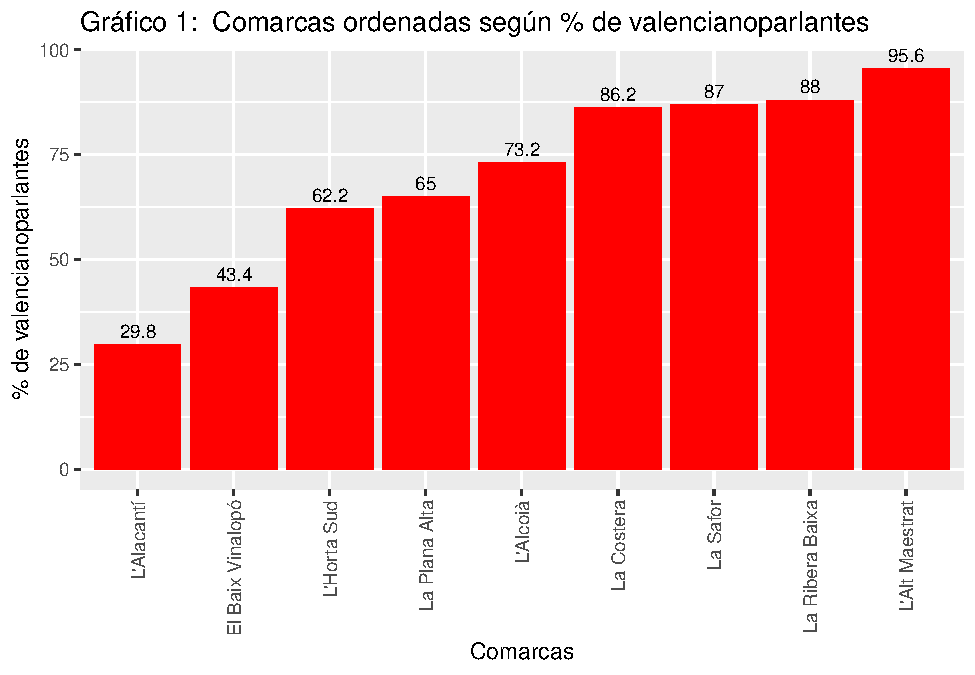
\includegraphics{votovalencianista-ea2023_page_files/figure-latex/ordenValencianoparlantes-1.pdf}
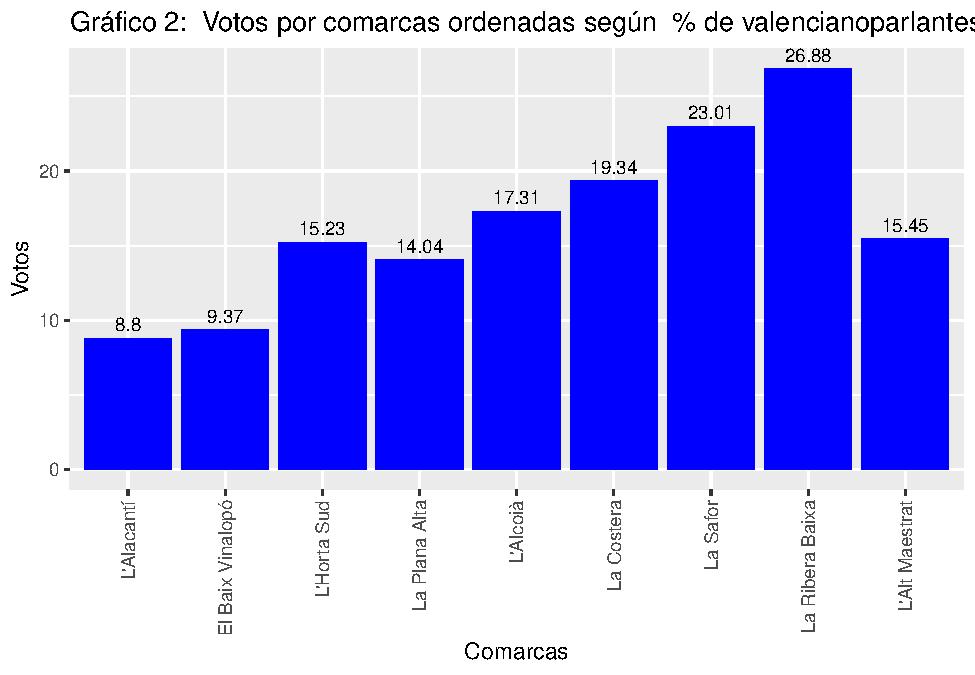
\includegraphics{votovalencianista-ea2023_page_files/figure-latex/ordenValencianoparlantes-2.pdf}

\begin{longtable}[]{@{}lrr@{}}
\caption{Tabla 5: Votos por comarcas ordenadas según \% de
valencianoparlantes}\tabularnewline
\toprule\noalign{}
Comarca & \% Votos & \% de valencianoparlantes \\
\midrule\noalign{}
\endfirsthead
\toprule\noalign{}
Comarca & \% Votos & \% de valencianoparlantes \\
\midrule\noalign{}
\endhead
\bottomrule\noalign{}
\endlastfoot
L'Alacantí & 8.80 & 29.8 \\
El Baix Vinalopó & 9.37 & 43.4 \\
L'Horta Sud & 15.23 & 62.2 \\
La Plana Alta & 14.04 & 65.0 \\
L'Alcoià & 17.31 & 73.2 \\
La Costera & 19.34 & 86.2 \\
La Safor & 23.01 & 87.0 \\
La Ribera Baixa & 26.88 & 88.0 \\
L'Alt Maestrat & 15.45 & 95.6 \\
\end{longtable}

\hypertarget{resultados-sobre-la-relaciuxf3n-causal-de-la-ruralidad-dendidad-poblacional}{%
\subsection{Resultados sobre la relación causal de la ruralidad
(dendidad
poblacional)}\label{resultados-sobre-la-relaciuxf3n-causal-de-la-ruralidad-dendidad-poblacional}}

En este apartado presentamos la matriz ordenada por el indicador
Habitantes por Km2 y dos gráficos obtenidos a partir de la tabla. De
forma que en el eje X siempre tendremos, en orden creciente, las
comarcas ordenadas por este indicador (Habitantes por Km2 por comarca) y
en el eje Y, el porcentaje de voto

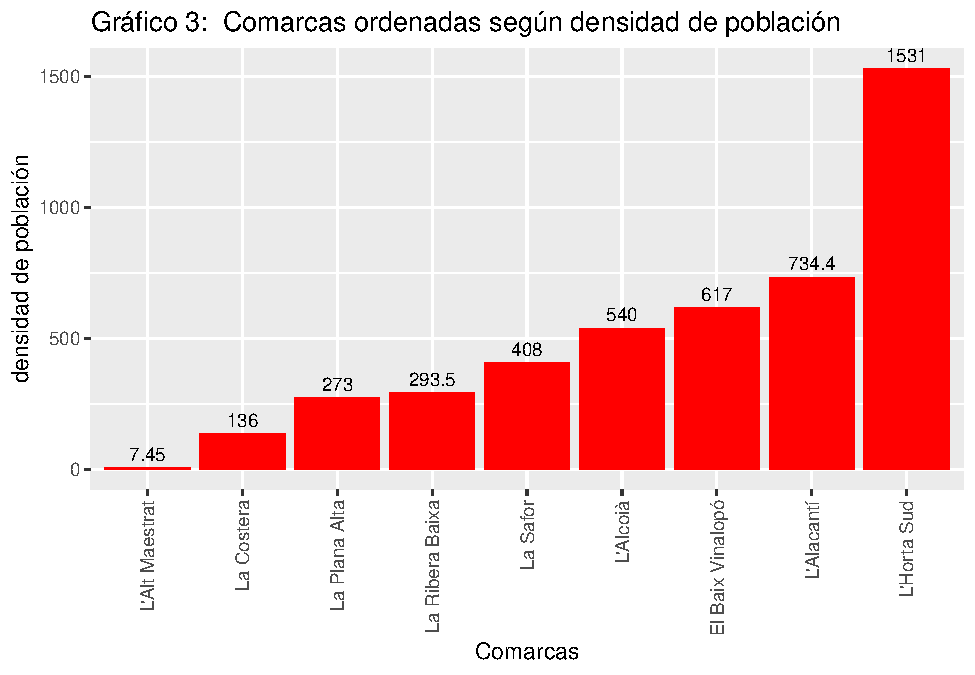
\includegraphics{votovalencianista-ea2023_page_files/figure-latex/ordenDensidadpoblacional-1.pdf}
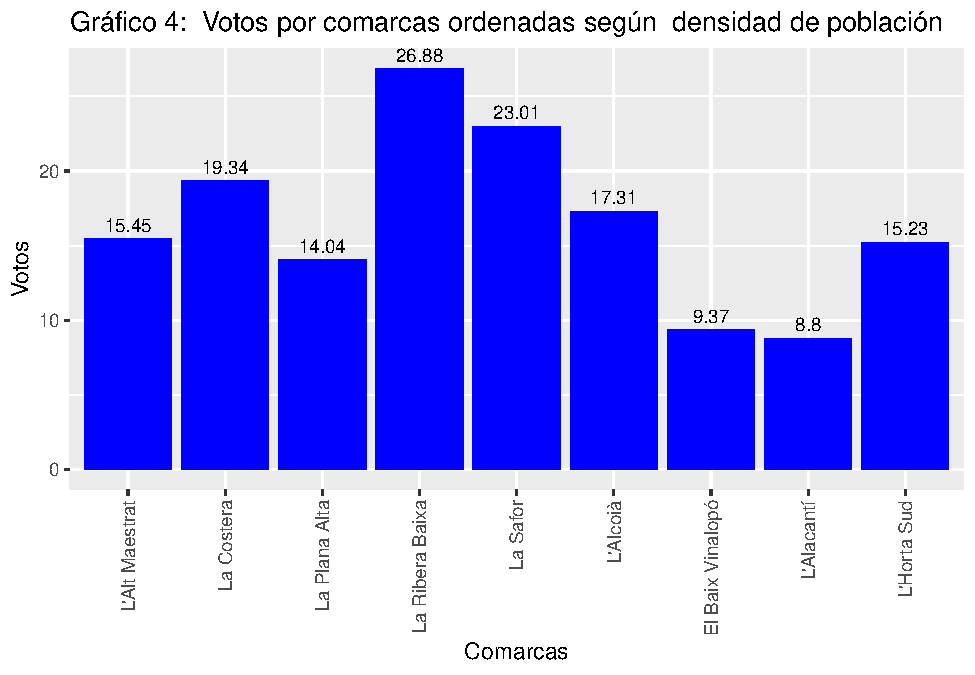
\includegraphics{votovalencianista-ea2023_page_files/figure-latex/ordenDensidadpoblacional-2.pdf}

\begin{longtable}[]{@{}lrr@{}}
\caption{Tabla 6: Votos por comarcas ordenadas según densidad de
población}\tabularnewline
\toprule\noalign{}
Comarca & \% Votos & densidad de población \\
\midrule\noalign{}
\endfirsthead
\toprule\noalign{}
Comarca & \% Votos & densidad de población \\
\midrule\noalign{}
\endhead
\bottomrule\noalign{}
\endlastfoot
L'Alt Maestrat & 15.45 & 7.45 \\
La Costera & 19.34 & 136.00 \\
La Plana Alta & 14.04 & 273.00 \\
La Ribera Baixa & 26.88 & 293.50 \\
La Safor & 23.01 & 408.00 \\
L'Alcoià & 17.31 & 540.00 \\
El Baix Vinalopó & 9.37 & 617.00 \\
L'Alacantí & 8.80 & 734.40 \\
L'Horta Sud & 15.23 & 1531.00 \\
\end{longtable}

\hypertarget{resultados-sobre-la-relaciuxf3n-causal-de-la-centralidad}{%
\subsection{Resultados sobre la relación causal de la
centralidad}\label{resultados-sobre-la-relaciuxf3n-causal-de-la-centralidad}}

Nos centramos en una primera parte en la Hipótesis 3, la que plantea la
distancia kilométrica entre comarca y la capital del País Valenciano
como causa posible de los votos a partidos valencianistas. En este
apartado presentamos la matriz ordenada por el indicador Km a València y
dos gráficos obtenidos a partir de la tabla. De forma que en el eje X
siempre tendremos, en orden creciente, las comarcas ordenadas por este
indicador (Km a València por comarca) y en el eje Y, el porcentaje de
voto.

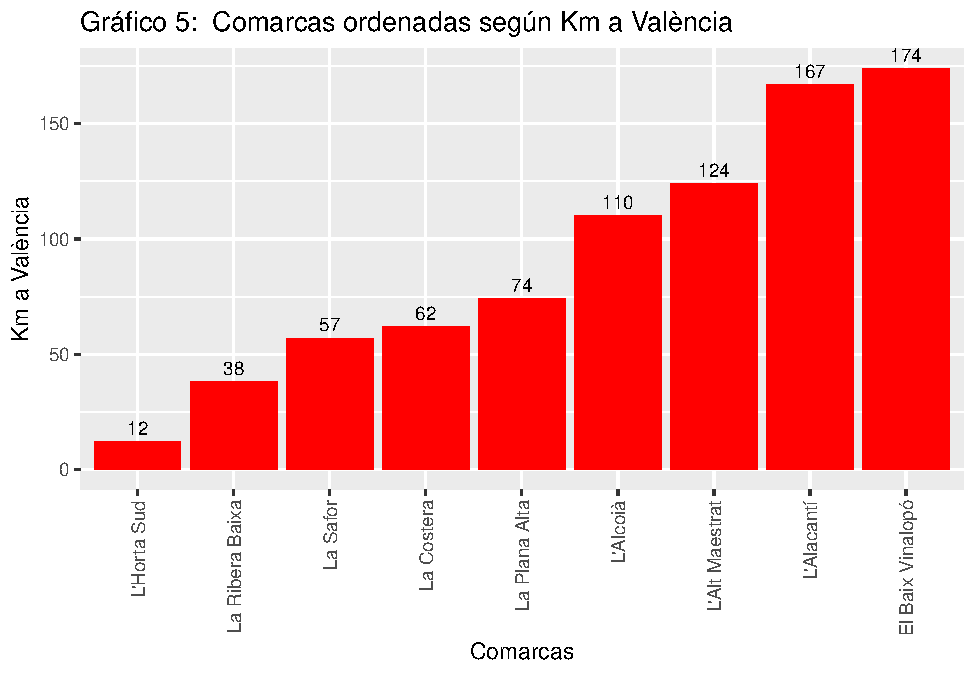
\includegraphics{votovalencianista-ea2023_page_files/figure-latex/ordenDistanciacapital-1.pdf}
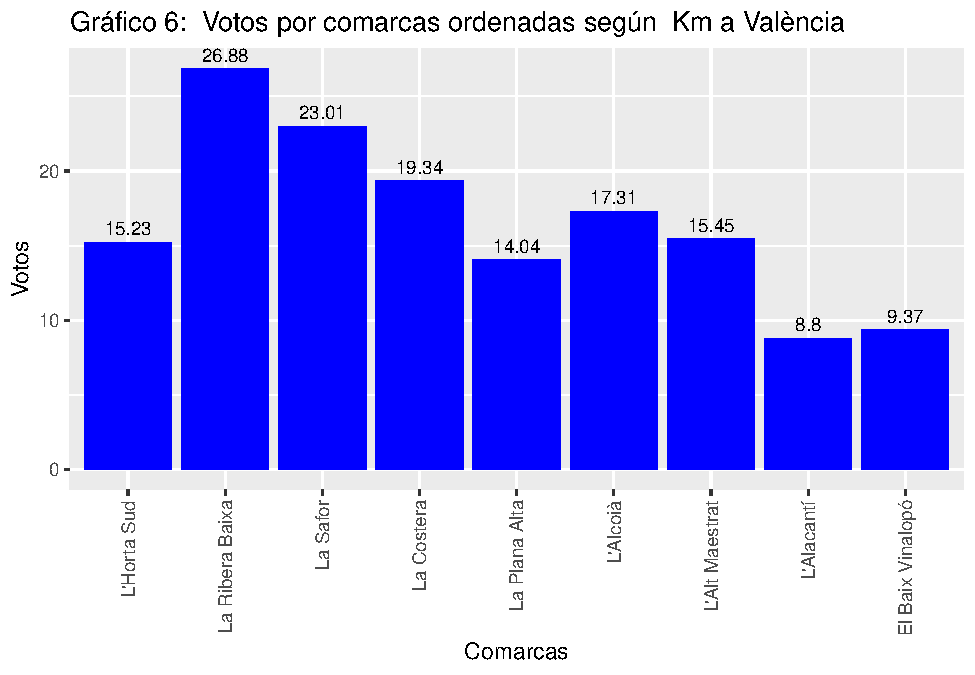
\includegraphics{votovalencianista-ea2023_page_files/figure-latex/ordenDistanciacapital-2.pdf}

\begin{longtable}[]{@{}lrr@{}}
\caption{Tabla 7: Votos por comarcas ordenadas según Km a
València}\tabularnewline
\toprule\noalign{}
Comarca & \% Votos & Km a València \\
\midrule\noalign{}
\endfirsthead
\toprule\noalign{}
Comarca & \% Votos & Km a València \\
\midrule\noalign{}
\endhead
\bottomrule\noalign{}
\endlastfoot
L'Horta Sud & 15.23 & 12 \\
La Ribera Baixa & 26.88 & 38 \\
La Safor & 23.01 & 57 \\
La Costera & 19.34 & 62 \\
La Plana Alta & 14.04 & 74 \\
L'Alcoià & 17.31 & 110 \\
L'Alt Maestrat & 15.45 & 124 \\
L'Alacantí & 8.80 & 167 \\
El Baix Vinalopó & 9.37 & 174 \\
\end{longtable}

La otra dimensión de la variable independiente de centralidad
corresponde a la Hipótesis 4, la que plantea la pertenencia de la
comarca a una división provincial u otra como causa de un mayor o menor
porcentaje de votos a partidos valencianistas. Vemos la matriz de
resultados clasificada por el indicador Provincia y, dentro de cada
clasificación, ordenada por el indicador de Km de Valencia. El siguiente
gráfico obtenido a partir de tabla anterior muestra visualmente la
diferencia de \% de votos para cada valor nominal.

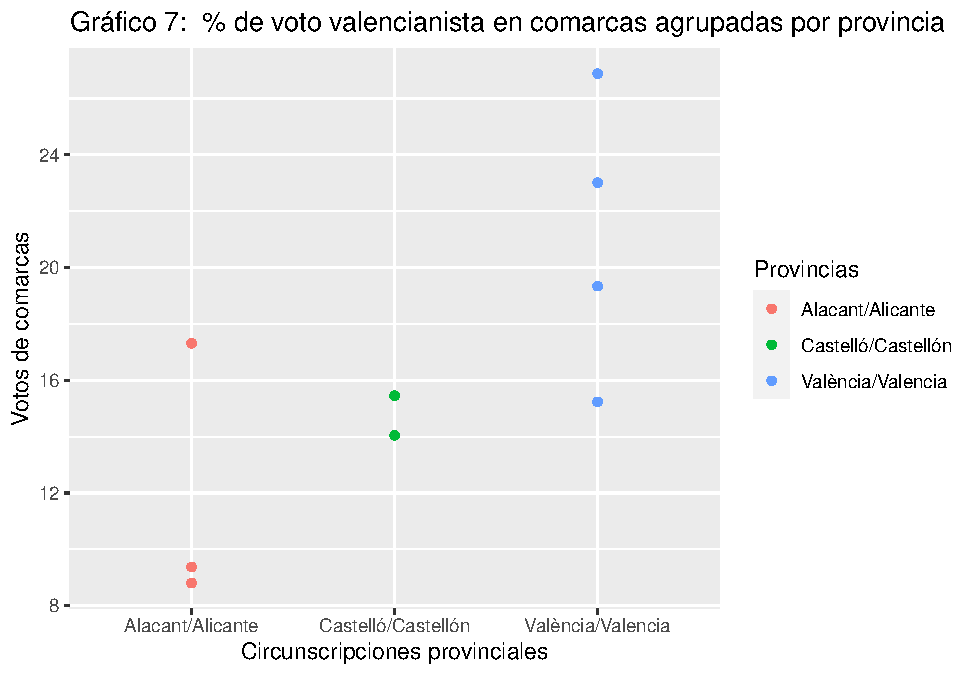
\includegraphics[width=0.8\linewidth,height=0.8\textheight]{votovalencianista-ea2023_page_files/figure-latex/funcionesGrafico2-1}

\begin{longtable}[]{@{}llr@{}}
\caption{Tabla 8: \% de voto valencianista en comarcas agrupadas por
provincia}\tabularnewline
\toprule\noalign{}
Provincia & Comarca & \% Votos \\
\midrule\noalign{}
\endfirsthead
\toprule\noalign{}
Provincia & Comarca & \% Votos \\
\midrule\noalign{}
\endhead
\bottomrule\noalign{}
\endlastfoot
Alacant/Alicante & El Baix Vinalopó & 9.37 \\
Alacant/Alicante & L'Alacantí & 8.80 \\
Alacant/Alicante & L'Alcoià & 17.31 \\
Castelló/Castellón & L'Alt Maestrat & 15.45 \\
Castelló/Castellón & La Plana Alta & 14.04 \\
València/Valencia & L'Horta Sud & 15.23 \\
València/Valencia & La Costera & 19.34 \\
València/Valencia & La Ribera Baixa & 26.88 \\
València/Valencia & La Safor & 23.01 \\
\end{longtable}

Obtener la media de votos por provincia de la Base de Datos ARGOS solo
requiere una sencilla consulta con lo que podemos hacer una comprobación
rápida nuestras medias.

\hypertarget{la-provuxedncia-como-variable-de-control}{%
\subsection{La província como variable de
control}\label{la-provuxedncia-como-variable-de-control}}

Como hemos visto, el concepto de centralidad, lo hemos operacionalizado
con dos indicadores, contemplando así dos dimensiones posibles de la
misma variable. Resulta interesante comprobar el efecto de cada una de
ellas de forma de forma independiente. Usaremos la variable de provincia
como variable de control manteniendo su valor constante (método
\emph{ceteris paribus}) y veremos cómo se comporta la variable
dependiente, el porcentaje de voto, en función de la otra variable
independiente (distancia kilométrica) entre la capital de cada comarca y
la capital de la región.

\textbf{Variable de control:} la variable independiente ``Provincia''.

\textbf{Variable independiente:} Distancia a la capital.

\hypertarget{centralidad-desde-la-provincia-de-alicante}{%
\subsubsection{Centralidad desde la provincia de
Alicante}\label{centralidad-desde-la-provincia-de-alicante}}

En este gráfico presentamos en el eje de abscisas las comarcas en orden
creciente de distancia desde su capital a València. En el eje de
ordenadas, tendremos el porcentaje total de votos valencianistas para la
provincia de Alicante.

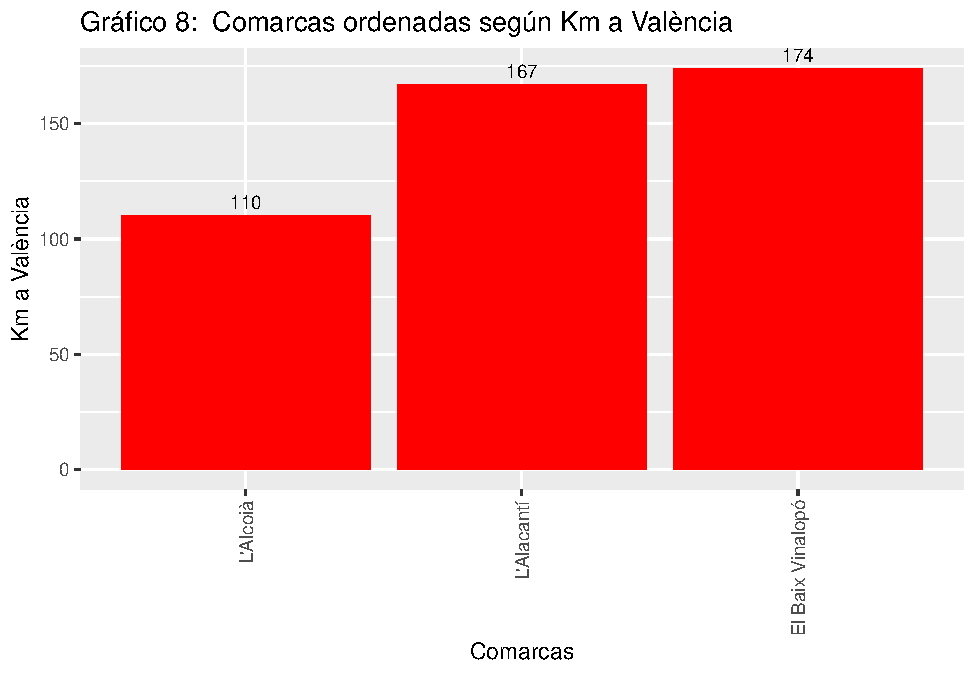
\includegraphics{votovalencianista-ea2023_page_files/figure-latex/ordenDistanciacapitalAlicante-1.pdf}
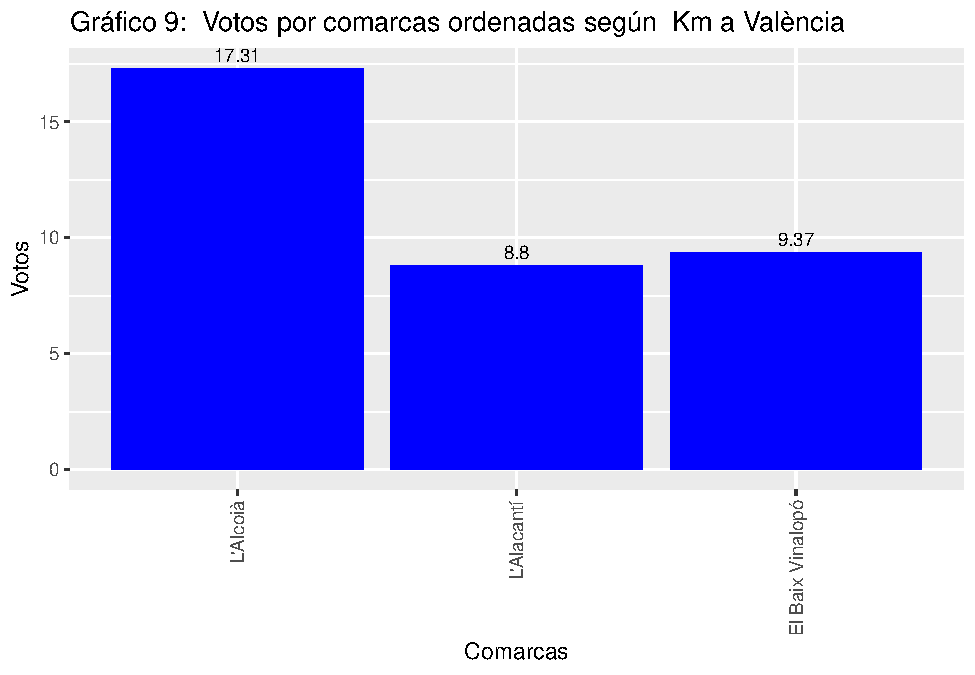
\includegraphics{votovalencianista-ea2023_page_files/figure-latex/ordenDistanciacapitalAlicante-2.pdf}

\begin{longtable}[]{@{}lrr@{}}
\caption{Tabla 9: Votos por comarcas ordenadas según Km a
València}\tabularnewline
\toprule\noalign{}
Comarca & \% Votos & Km a València \\
\midrule\noalign{}
\endfirsthead
\toprule\noalign{}
Comarca & \% Votos & Km a València \\
\midrule\noalign{}
\endhead
\bottomrule\noalign{}
\endlastfoot
L'Alcoià & 17.31 & 110 \\
L'Alacantí & 8.80 & 167 \\
El Baix Vinalopó & 9.37 & 174 \\
\end{longtable}

\hypertarget{la-centralidad-desde-la-provincia-de-castelluxf3n}{%
\subsubsection{La centralidad desde la provincia de
Castellón}\label{la-centralidad-desde-la-provincia-de-castelluxf3n}}

En este gráfico presentamos en el eje de abscisas las comarcas en orden
creciente de distancia desde su capital a València. En el eje de
ordenadas, tendremos el porcentaje total de votos valencianistas para la
provincia de Castellón.

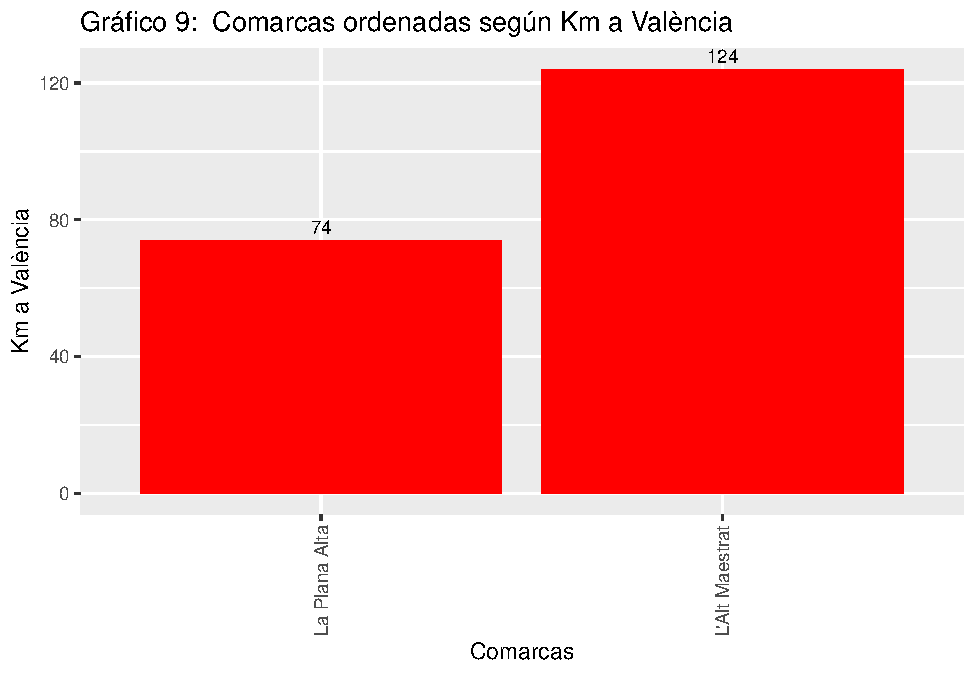
\includegraphics{votovalencianista-ea2023_page_files/figure-latex/ordenDistanciacapitalCastellon-1.pdf}
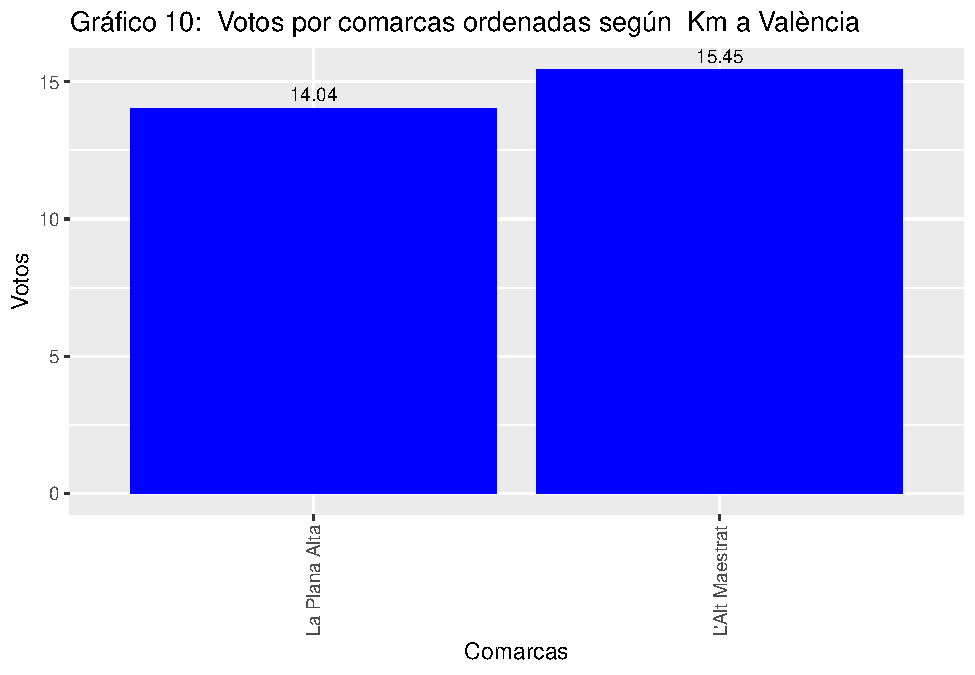
\includegraphics{votovalencianista-ea2023_page_files/figure-latex/ordenDistanciacapitalCastellon-2.pdf}

\begin{longtable}[]{@{}lrr@{}}
\caption{Tabla 11: Votos por comarcas ordenadas según Km a
València}\tabularnewline
\toprule\noalign{}
Comarca & \% Votos & Km a València \\
\midrule\noalign{}
\endfirsthead
\toprule\noalign{}
Comarca & \% Votos & Km a València \\
\midrule\noalign{}
\endhead
\bottomrule\noalign{}
\endlastfoot
La Plana Alta & 14.04 & 74 \\
L'Alt Maestrat & 15.45 & 124 \\
\end{longtable}

\hypertarget{la-centralidad-desde-la-provincia-de-valuxe8ncia}{%
\subsubsection{La centralidad desde la provincia de
València}\label{la-centralidad-desde-la-provincia-de-valuxe8ncia}}

En este gráfico presentamos en el eje de abscisas las comarcas en orden
creciente de distancia desde su capital a València. En el eje de
ordenadas, tendremos el porcentaje total de votos valencianistas para la
provincia de Valencia.

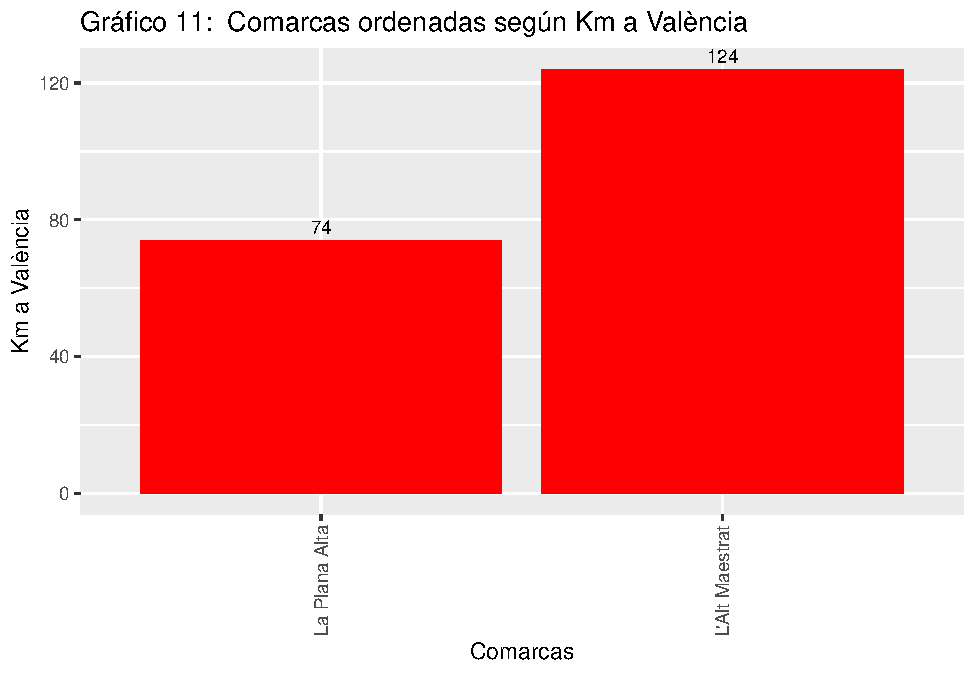
\includegraphics{votovalencianista-ea2023_page_files/figure-latex/ordenDistanciacapitalValencia-1.pdf}
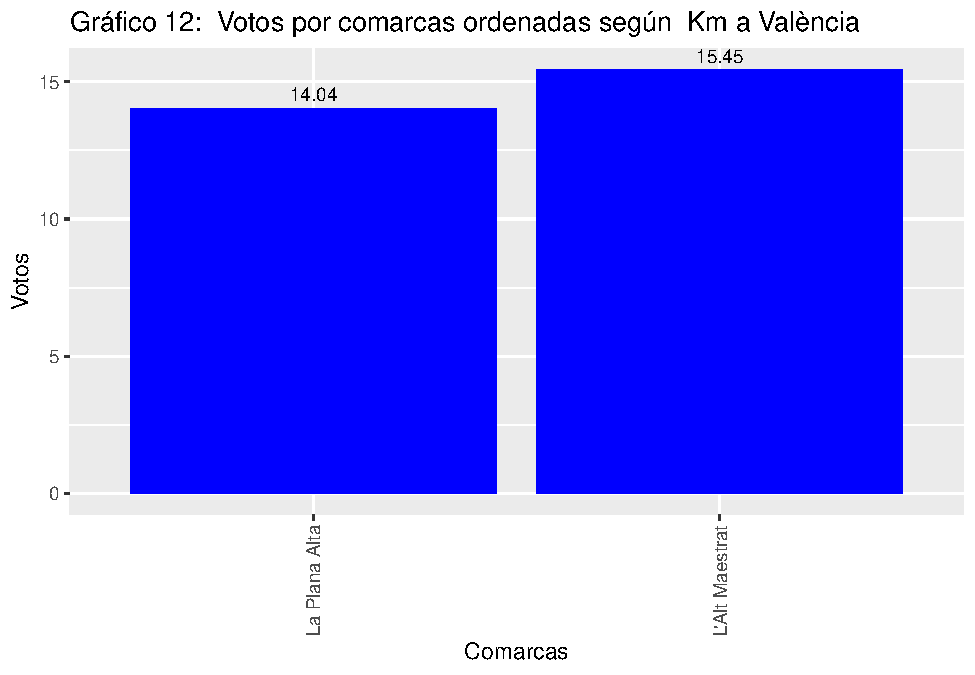
\includegraphics{votovalencianista-ea2023_page_files/figure-latex/ordenDistanciacapitalValencia-2.pdf}

\begin{longtable}[]{@{}lrr@{}}
\caption{Tabla 12: Votos por comarcas ordenadas según Km a
València}\tabularnewline
\toprule\noalign{}
Comarca & \% Votos & Km a València \\
\midrule\noalign{}
\endfirsthead
\toprule\noalign{}
Comarca & \% Votos & Km a València \\
\midrule\noalign{}
\endhead
\bottomrule\noalign{}
\endlastfoot
La Plana Alta & 14.04 & 74 \\
L'Alt Maestrat & 15.45 & 124 \\
\end{longtable}

El uso de la variable de control Provincia nos ha permitido averiguar
que, si bien inicialmente, podíamos haber deducido que a mayor distancia
a la capital, menor era el voto valencianista en toda la Comunidad (ver
Gráfico 6) realmente esto no era así.

Mediante el método \textbf{ceteris paribus} ( \textbf{variable de
control}: circunscripción provincial) hemos averiguado que esta
hipótesis de trabajo que señalaba al indicador de distancia a la capital
como causa de un menor voto valencianista (a mayor distancia, menor \%
de votos) se cumpliría, en todo caso, solo en las comarcas del sur, en
la provincia de Alicante (ver Gráfico 7). De hecho, en las comarcas de
Valencia y Castelló se llega a aprceia el efecto contrario (ver Gráficos
9 y Gráfico 11)

\hypertarget{conclusiones}{%
\section{10.CONCLUSIONES}\label{conclusiones}}

Respecto al diferente porcentaje de voto por comarcas a Compromís, como
única fuerza valencianista que obtuvo un porcentaje de votos superior al
2\% en las elecciones autonómicas del 2023, podemos concluir que:

\begin{enumerate}
\def\labelenumi{\arabic{enumi}.}
\item
  Hay una relación causal entre el predominio del idioma valenciano en
  la comarca y el voto a Compromís: a mayor predomino, más votos. Aun
  así, en comarcas castellanohablantes Compromís obtiene valores por
  encima del 10\%. Se cumple la Hipótesis 1.
\item
  No se puede establecer una relación de causalidad entre ruralidad de
  la comarca y este voto valencianista. La Hipótesis 2 no se cumple
\item
  Existe una causalidad entre la distancia a la capital y el voto
  valencianista en la Provincia de Alicante; en las comarcas más
  alejadas de Valencia se obtienen menos votos. En la provincia de
  Valencia, esta causalidad opera en sentido contrario: comarcas más
  alejadas del Cap i casal votan más a Compromís. En Castellón tampoco
  se cumple la hipótesis inicial. La Hipótesis de trabajo 3 no se cumple
  con lo que la hipótesis 3 no se cumple como tal.
\item
  La pertenencia a una provincia u otra sí que explica una tendencia al
  voto valencianista. Existe un mayor voto a Compromís en las comarcas
  de la provincia de Valencia y un menor voto en las de Alicante,
  quedando Castellón en una posición intermedia. La Hipótesis de trabajo
  4 si cumple.
\end{enumerate}

\hypertarget{lista-de-referencias-bibliogruxe1ficas}{%
\section{11.LISTA DE REFERENCIAS
BIBLIOGRÁFICAS}\label{lista-de-referencias-bibliogruxe1ficas}}

\begin{itemize}
\tightlist
\item
  FUKUYAMA, Francis 2019, Identidad. Barcelona: Editorial Planeta.
\item
  FUSTER, J. 1988 Nosaltres els valencians. València; Edicions 3 i 4
\item
  LIPSET, Seymour y ROKKAN, Stein, LIPSET, Estructuras de división,
  sistemas de partidos y alineamientos electorales, traducción en
  español en Diez textos básicos de ciencia política, Ariel, Barcelona
  2001.
\item
  MIRA, Joan F. 2005. Crítica de la nació pura. València: Edicions 3 i
  4.
\item
  RODRÍGUEZ-AGUILERA, C. Manual de partidos políticos. Barcelona:
  Huygens Editorial.
\item
  SARTORI, G. 1992. Partidos y sistemas de partidos. Madrid.
\end{itemize}

\hypertarget{otros-recursos}{%
\section{12. OTROS RECURSOS}\label{otros-recursos}}

\begin{itemize}
\tightlist
\item
  ARGOS. Base de datos de resultado electorales de la Generalitat
  Valenciana. \url{https://www.argos.gva.es}
\item
  Encuestas sobre la situación del valenciano. Dirección General de
  Política Lingüística.
  \url{https://ceice.gva.es/va/web/dgplgm/enquestes-situacio-valencia}
\item
  Institut Valencià d'Estadística. Generalitat Valenciana.
  \url{https://pegv.gva.es/auto/scpd/web/DBCV/DBCV_2021_C.pdf}
\item
  Instituto Nacional de Estadística \url{https://www.ine.es}
\item
  Portal de Dades Obertes de la Generalitat Valenciana.
  \url{https://portaldadesobertes.gva.es/va/}
\end{itemize}

\hypertarget{anexo.-r-markdown}{%
\section{13. ANEXO. R Markdown}\label{anexo.-r-markdown}}

El presente documento ha sido editado en R Markdown. Los datos obtenidos
obtenidos de las fuentes citadas en el anterior apartado han sido
procesados mediante el lenguaje de programación R. Tanto para el cálculo
de valores numéricos como la elaboración e impresión de tablas,
diagramas y gráficos. Veamos por orden de uso en el documento los
diferentes \emph{chunks} de R integrados en el documento.

Se ha insertado en este anexo los valores \emph{val=FALSE} para evitar
la ejecución del código r y el valor \emph{echo=TRUE} para que sea
visible.

\hypertarget{instalaciuxf3n-de-paquetes-y-carga-de-libreruxedas-requeridas}{%
\subsection{Instalación de paquetes y carga de librerías
requeridas}\label{instalaciuxf3n-de-paquetes-y-carga-de-libreruxedas-requeridas}}

\begin{Shaded}
\begin{Highlighting}[]
\CommentTok{\# Requisitos previos. Paquetes y librerías}
\ControlFlowTok{if}\NormalTok{ (}\SpecialCharTok{!}\FunctionTok{require}\NormalTok{(}\StringTok{"dplyr"}\NormalTok{)) \{}\FunctionTok{install.packages}\NormalTok{(}\StringTok{"dplyr"}\NormalTok{)\}}
\ControlFlowTok{if}\NormalTok{ (}\SpecialCharTok{!}\FunctionTok{require}\NormalTok{(}\StringTok{"stringr"}\NormalTok{)) \{}\FunctionTok{install.packages}\NormalTok{(}\StringTok{"stringr"}\NormalTok{)\}}
\ControlFlowTok{if}\NormalTok{ (}\SpecialCharTok{!}\FunctionTok{require}\NormalTok{(}\StringTok{"tidyverse"}\NormalTok{))\{}\FunctionTok{install.packages}\NormalTok{(}\StringTok{"tidyverse"}\NormalTok{)\}}
\FunctionTok{library}\NormalTok{(stringr)}
\FunctionTok{library}\NormalTok{(dplyr)}
\FunctionTok{library}\NormalTok{(ggplot2)}
\FunctionTok{library}\NormalTok{(tidyverse)}
\end{Highlighting}
\end{Shaded}

\hypertarget{funciones-para-imprimir-2-gruxe1ficos-y-1-tabla}{%
\subsection{Funciones para imprimir 2 gráficos y 1
tabla}\label{funciones-para-imprimir-2-gruxe1ficos-y-1-tabla}}

\begin{Shaded}
\begin{Highlighting}[]
\CommentTok{\# F. IMPRESION GRAFICO DE BARRAS A PARTIR DE UN DATA FRAME}
\NormalTok{f\_graficoBarres}\OtherTok{\textless{}{-}}\ControlFlowTok{function}\NormalTok{(dfplot)\{}
 
\NormalTok{gr\_voto}\OtherTok{\textless{}{-}}\FunctionTok{ggplot}\NormalTok{(dfplot,}\FunctionTok{aes}\NormalTok{(}\AttributeTok{x=}\FunctionTok{factor}\NormalTok{(x,}\AttributeTok{levels=}\FunctionTok{c}\NormalTok{(x)),}\AttributeTok{y=}\NormalTok{y1))}\SpecialCharTok{+}
   \FunctionTok{geom\_bar}\NormalTok{(}\AttributeTok{stat =} \StringTok{"identity"}\NormalTok{, }\AttributeTok{fill =}\StringTok{"blue"}\NormalTok{, }\AttributeTok{position =} \StringTok{"dodge"}\NormalTok{)}\SpecialCharTok{+}
   \FunctionTok{theme}\NormalTok{(}\AttributeTok{axis.text.x =} \FunctionTok{element\_text}\NormalTok{(}\AttributeTok{angle =} \DecValTok{90}\NormalTok{, }\AttributeTok{vjust =} \FloatTok{0.5}\NormalTok{, }\AttributeTok{hjust =} \DecValTok{1}\NormalTok{))}\SpecialCharTok{+}
   \FunctionTok{labs}\NormalTok{(}\AttributeTok{x =} \StringTok{"Comarcas"}\NormalTok{, }\AttributeTok{y =} \StringTok{"Votos"}\NormalTok{, }\AttributeTok{title =} \FunctionTok{paste}\NormalTok{(}\FunctionTok{attr}\NormalTok{(dfplot,}\StringTok{"grafico2"}\NormalTok{),}\StringTok{"Votos por comarcas ordenadas según "}\NormalTok{,}\FunctionTok{attr}\NormalTok{(dfplot,}\StringTok{"criterio"}\NormalTok{)))}\SpecialCharTok{+}
   \FunctionTok{geom\_text}\NormalTok{(}\FunctionTok{aes}\NormalTok{(}\AttributeTok{label =}\NormalTok{ y1), }\AttributeTok{vjust =} \SpecialCharTok{{-}}\FloatTok{0.5}\NormalTok{, }\AttributeTok{color =} \StringTok{"black"}\NormalTok{, }\AttributeTok{size =} \DecValTok{3}\NormalTok{) }

\NormalTok{gr\_criterio}\OtherTok{\textless{}{-}}\FunctionTok{ggplot}\NormalTok{(dfplot,}\FunctionTok{aes}\NormalTok{(}\AttributeTok{x=}\FunctionTok{factor}\NormalTok{(x,}\AttributeTok{levels=}\FunctionTok{c}\NormalTok{(x)),}\AttributeTok{y=}\NormalTok{y2))}\SpecialCharTok{+}
   \FunctionTok{geom\_bar}\NormalTok{(}\AttributeTok{stat =} \StringTok{"identity"}\NormalTok{, }\AttributeTok{fill =} \StringTok{"red"}\NormalTok{, }\AttributeTok{position =} \StringTok{"dodge"}\NormalTok{)}\SpecialCharTok{+}
   \FunctionTok{theme}\NormalTok{(}\AttributeTok{axis.text.x =} \FunctionTok{element\_text}\NormalTok{(}\AttributeTok{angle =} \DecValTok{90}\NormalTok{, }\AttributeTok{vjust =} \FloatTok{0.5}\NormalTok{, }\AttributeTok{hjust =} \DecValTok{1}\NormalTok{))}\SpecialCharTok{+}
   \FunctionTok{labs}\NormalTok{(}\AttributeTok{x =} \StringTok{"Comarcas"}\NormalTok{, }\AttributeTok{y =} \FunctionTok{attr}\NormalTok{(dfplot,}\StringTok{"criterio"}\NormalTok{), }\AttributeTok{title =} \FunctionTok{paste}\NormalTok{(}\FunctionTok{attr}\NormalTok{(dfplot,}\StringTok{"grafico1"}\NormalTok{),}\StringTok{"Comarcas ordenadas según"}\NormalTok{,}\FunctionTok{attr}\NormalTok{(dfplot,}\StringTok{"criterio"}\NormalTok{)))}\SpecialCharTok{+}
   \FunctionTok{geom\_text}\NormalTok{(}\FunctionTok{aes}\NormalTok{(}\AttributeTok{label =}\NormalTok{ y2), }\AttributeTok{vjust =} \SpecialCharTok{{-}}\FloatTok{0.5}\NormalTok{, }\AttributeTok{color =} \StringTok{"black"}\NormalTok{, }\AttributeTok{size =} \DecValTok{3}\NormalTok{) }
\CommentTok{\#Vemos el criterio como evoluciona en las comarcas}
\FunctionTok{print}\NormalTok{(gr\_criterio)}
\CommentTok{\#Vemos el resultado de votos según este criterio ( gráfico y tabla)}
\FunctionTok{print}\NormalTok{(gr\_voto)}
  \CommentTok{\# imprimir tabla asociada}
\FunctionTok{colnames}\NormalTok{(dfplot) }\OtherTok{\textless{}{-}} \FunctionTok{c}\NormalTok{(}\StringTok{"Comarca"}\NormalTok{, }\StringTok{"\% Votos"}\NormalTok{,}\FunctionTok{attr}\NormalTok{(dfplot,}\StringTok{"criterio"}\NormalTok{))}
\NormalTok{knitr}\SpecialCharTok{::}\FunctionTok{kable}\NormalTok{(dfplot, }\AttributeTok{caption =} \FunctionTok{paste}\NormalTok{(}\FunctionTok{attr}\NormalTok{(dfplot,}\StringTok{"tabla"}\NormalTok{),}\StringTok{"Votos por comarcas ordenadas según "}\NormalTok{,}\FunctionTok{attr}\NormalTok{(dfplot,}\StringTok{"criterio"}\NormalTok{)))}
\NormalTok{  \}}
\end{Highlighting}
\end{Shaded}

\hypertarget{modelo-teuxf3rico-de-la-investigaciuxf3n-1}{%
\subsection{Modelo teórico de la
investigación}\label{modelo-teuxf3rico-de-la-investigaciuxf3n-1}}

\begin{Shaded}
\begin{Highlighting}[]
\CommentTok{\#DIAGRAMA QUE REPRESENTA EL MODELO TEÓRICO DE LA INVESTIGACIÓN}
\FunctionTok{library}\NormalTok{(}\StringTok{"DiagrammeR"}\NormalTok{)}
\FunctionTok{grViz}\NormalTok{(}\StringTok{"}
\StringTok{      digraph test \{}
\StringTok{      labelloc=\textquotesingle{}t\textquotesingle{}}
\StringTok{      label=\textquotesingle{}Figura 1: Modelo teórico de investigación\textquotesingle{}}
\StringTok{      fontsize=14}
\StringTok{      fontname = \textquotesingle{}DejaVu Sans\textquotesingle{}}
\StringTok{      }
\StringTok{        rankdir= LR}
\StringTok{        node [shape = box, width = 0.7, height = 0.4, style = filled, color = lightblue, labelloc = c, fixedsize = true, spacing=0.3,fontname = \textquotesingle{}DejaVu Sans\textquotesingle{}, fontsize = 4]}
\StringTok{        A[label =\textquotesingle{}Predominio}\SpecialCharTok{\textbackslash{}n}\StringTok{lingüístico}\SpecialCharTok{\textbackslash{}n}\StringTok{del valenciano\textquotesingle{}]}
\StringTok{        B[label=\textquotesingle{}Centralidad\textquotesingle{}]}
\StringTok{        C[label=\textquotesingle{}Ruralidad\textquotesingle{}]}
\StringTok{        node [shape = box, width = 1,fontname = \textquotesingle{}sans\textquotesingle{}, fontsize = 6]}
\StringTok{        D[label =\textquotesingle{}Voto a partidos}\SpecialCharTok{\textbackslash{}n}\StringTok{ valencianistas\textquotesingle{}];}
\StringTok{        A {-}\textgreater{} D [label=\textquotesingle{}+\textquotesingle{}, arrowsize=0.4]}
\StringTok{        B {-}\textgreater{} D [label=\textquotesingle{}+\textquotesingle{}, arrowsize=0.4]}
\StringTok{        C {-}\textgreater{} D [label=\textquotesingle{}+\textquotesingle{}, arrowsize=0.4]}
\StringTok{      \{ rank = same; A; B; C \}}
\StringTok{      \}}
\StringTok{ "}\NormalTok{)}
\end{Highlighting}
\end{Shaded}

\hypertarget{obtenciuxf3n-de-data-frame-a-partir-de-los-datos-abiertos}{%
\subsection{Obtención de data frame a partir de los datos
abiertos}\label{obtenciuxf3n-de-data-frame-a-partir-de-los-datos-abiertos}}

A partir de ficheros CSV obtenidos de las diversas fuentes citadas, se
procesan en R para crear dos Data Frame (Universo y Muestra ). Las
columnas de estos corresponderan a las variables independientes y la
dependiente. El Universo contemplará todas la comarcas del País
Valenciano mientras que la Muestra solo las seleccionadas.

\begin{Shaded}
\begin{Highlighting}[]
\CommentTok{\# LECTURA DE LOS FICHEROS csv DEL OPEN DATA DE LA GV CON LOS RESULTADOS A NIVEL DE AGREGACIÓN DE MESA ELECTORAL}
\CommentTok{\# VAMOS A CERAR UN FICHERO CON EL \%DE VOTO SOBRE CANDIDATURA A LAS CANDIDATURAS VALENCIANISTAS A NIVEL DE AGREGACIÓN COMARCAL QUE INDIQUE:}
\CommentTok{\# PROVINCIA, COMARCA, PORCENTAJE DE VOTO}

\NormalTok{df0}\OtherTok{\textless{}{-}}\FunctionTok{read.csv}\NormalTok{(}\StringTok{"CSV/resultados{-}elecciones{-}autonomicas{-}1{-}2023.csv"}\NormalTok{, }\AttributeTok{fileEncoding=}\StringTok{"latin3"}\NormalTok{)}
\CommentTok{\# Paso 1: Eliminamos las líneas de "Residentes ausentes puesto que no pertenecen a ninguna comarca.}
\CommentTok{\#nrow(df0[df0$Districte==99,]) \#Vemos cuantoss hay}
\CommentTok{\# nrow(df0[df0$Desc\_Comarca=="",])}
\NormalTok{df0}\OtherTok{\textless{}{-}}\NormalTok{df0[}\SpecialCharTok{!}\NormalTok{df0}\SpecialCharTok{$}\NormalTok{Desc\_Comarca}\SpecialCharTok{==}\StringTok{""}\NormalTok{,] }

\CommentTok{\# Paso 2: Agrupamos a nivel de mesa para poder obtener los datos que se repiten en cada fila (candidatura) por mesa y necesitaremos (Voto en blanco y Voto nulo )}
\FunctionTok{suppressMessages}\NormalTok{(df1}\OtherTok{\textless{}{-}}\FunctionTok{subset}\NormalTok{(df0,}\AttributeTok{select=}\FunctionTok{c}\NormalTok{(Desc\_Prov,Desc\_Comarca,Desc\_municipi,Districte,Secció,Mesa,VOTANTS,V\_NULS,V\_BLANC))}\SpecialCharTok{\%\textgreater{}\%}\FunctionTok{group\_by}\NormalTok{(Desc\_Prov,Desc\_Comarca,Desc\_municipi,Districte,Secció,Mesa) }\SpecialCharTok{\%\textgreater{}\%}\FunctionTok{summarise}\NormalTok{(}\AttributeTok{Blancos=}\FunctionTok{unique}\NormalTok{(V\_BLANC),}\AttributeTok{Nulos=}\FunctionTok{first}\NormalTok{(V\_NULS)))}

\CommentTok{\# Paso 3: Ahora sumando estos valores únicos por mesa ya podemos obtener el total de vOto en blanco y nulo por comarca}
\FunctionTok{suppressMessages}\NormalTok{(df2}\OtherTok{\textless{}{-}}\NormalTok{df1}\SpecialCharTok{\%\textgreater{}\%}\FunctionTok{group\_by}\NormalTok{(Desc\_Prov,Desc\_Comarca)}\SpecialCharTok{\%\textgreater{}\%}\FunctionTok{summarise}\NormalTok{(}\AttributeTok{Blancos=}\FunctionTok{sum}\NormalTok{(Blancos),}\AttributeTok{Nulos=}\FunctionTok{sum}\NormalTok{(Nulos)))}

\CommentTok{\# Paso 4: Agrupamos a nivel de comarca y sumamos los votos de todas las filas a cualquier partido. Voto a candidatura}
\FunctionTok{suppressMessages}\NormalTok{(df3}\OtherTok{\textless{}{-}}\NormalTok{df0}\SpecialCharTok{\%\textgreater{}\%} \FunctionTok{group\_by}\NormalTok{(Desc\_Prov,Desc\_Comarca) }\SpecialCharTok{\%\textgreater{}\%}\FunctionTok{summarise}\NormalTok{(}\AttributeTok{VotosCandidatura=}\FunctionTok{sum}\NormalTok{(V\_CAND)))}

\CommentTok{\# Paso 5: Agrupamos a nivel de comarca, filtrando por la candidatura 3 (Compromís) y sumamos usu votos}
\FunctionTok{suppressMessages}\NormalTok{(df4}\OtherTok{\textless{}{-}}\FunctionTok{subset}\NormalTok{(df0,df0}\SpecialCharTok{$}\NormalTok{CODI\_CANDIDATURA}\SpecialCharTok{==}\DecValTok{3}\NormalTok{) }\SpecialCharTok{\%\textgreater{}\%} \FunctionTok{group\_by}\NormalTok{(Desc\_Prov,Desc\_Comarca)}\SpecialCharTok{\%\textgreater{}\%}\FunctionTok{summarise}\NormalTok{(}\AttributeTok{VotoValencianista=}\FunctionTok{sum}\NormalTok{(V\_CAND)))}

\CommentTok{\# Paso 6: Unimos los dos data frame. La opción ,{-}1] evita la duplicación de columnas}
\NormalTok{dfMatrizInicial}\OtherTok{\textless{}{-}}\FunctionTok{merge}\NormalTok{(df2, df3[,}\SpecialCharTok{{-}}\DecValTok{1}\NormalTok{], }\AttributeTok{by =} \StringTok{"Desc\_Comarca"}\NormalTok{, }\AttributeTok{all =} \ConstantTok{TRUE}\NormalTok{)}
\NormalTok{dfMatrizInicial}\OtherTok{\textless{}{-}}\FunctionTok{merge}\NormalTok{(dfMatrizInicial, df4[,}\SpecialCharTok{{-}}\DecValTok{1}\NormalTok{], }\AttributeTok{by =} \StringTok{"Desc\_Comarca"}\NormalTok{, }\AttributeTok{all =} \ConstantTok{TRUE}\NormalTok{)}

\CommentTok{\# PAso 7: Creamos la primera matriz con porcentajes de voto valencianista por comarca}
\NormalTok{df\_votoycomarcas}\OtherTok{\textless{}{-}}\FunctionTok{data.frame}\NormalTok{(}\AttributeTok{Circunsc.=}\NormalTok{dfMatrizInicial}\SpecialCharTok{$}\NormalTok{Desc\_Prov,}
                            \AttributeTok{Comarca=}\NormalTok{dfMatrizInicial}\SpecialCharTok{$}\NormalTok{Desc\_Comarca,}
                            \AttributeTok{PorcVotoValencianista=}\FunctionTok{round}\NormalTok{(dfMatrizInicial}\SpecialCharTok{$}\NormalTok{VotoValencianista}\SpecialCharTok{*}\DecValTok{100}\SpecialCharTok{/}\NormalTok{dfMatrizInicial}\SpecialCharTok{$}\NormalTok{VotosCandidatura,}\DecValTok{2}\NormalTok{))}
\CommentTok{\#Este dataframe. df\_votoycomarcas, lo usaremos en el siguiente chunck fusionándolo con los datraframes obtenidos de los otros datos (lengua, distancia, densidad poblacional...)}
\end{Highlighting}
\end{Shaded}

\begin{Shaded}
\begin{Highlighting}[]
\NormalTok{df\_regionesycomarcas}\OtherTok{\textless{}{-}}\FunctionTok{read.csv}\NormalTok{(}\StringTok{"CSV/Regionesycomarcas.csv"}\NormalTok{,}\AttributeTok{dec=}\StringTok{","}\NormalTok{)}
\NormalTok{df\_densidad}\OtherTok{\textless{}{-}}\FunctionTok{read.csv}\NormalTok{(}\StringTok{"CSV/Densidadycomarcas.csv"}\NormalTok{,}\AttributeTok{dec=}\StringTok{","}\NormalTok{)}
\NormalTok{df\_distancia}\OtherTok{\textless{}{-}}\FunctionTok{read.csv}\NormalTok{(}\StringTok{"CSV/Distanciaycomarcas.csv"}\NormalTok{,}\AttributeTok{dec=}\StringTok{","}\NormalTok{)}

\CommentTok{\# Creamos el dataframe de todos los datos. Universo = todas las comarcas}
\NormalTok{df\_universo}\OtherTok{\textless{}{-}}\FunctionTok{merge}\NormalTok{(df\_votoycomarcas, df\_densidad[,}\SpecialCharTok{{-}}\DecValTok{1}\NormalTok{],}\AttributeTok{by=}\StringTok{"Comarca"}\NormalTok{)}
\NormalTok{df\_universo}\OtherTok{\textless{}{-}}\FunctionTok{merge}\NormalTok{(df\_universo, df\_distancia[,}\SpecialCharTok{{-}}\DecValTok{1}\NormalTok{],}\AttributeTok{by=}\StringTok{"Comarca"}\NormalTok{)}
\NormalTok{df\_universo}\OtherTok{\textless{}{-}}\FunctionTok{merge}\NormalTok{(df\_universo, df\_regionesycomarcas[,}\SpecialCharTok{{-}}\DecValTok{1}\NormalTok{],}\AttributeTok{by=}\StringTok{"Comarca"}\NormalTok{)}

\CommentTok{\# Leemos el un csv con las comarcas que queremos estudiar (muestra.csv)}
\NormalTok{df\_indiceMuestra}\OtherTok{\textless{}{-}}\FunctionTok{read.csv}\NormalTok{(}\StringTok{"CSV/Muestra.csv"}\NormalTok{)}

\CommentTok{\# Filtramos del Universo seleccionando solo las comarcas de nuestra muestra. df\_muestra será la MATRIZ de DATOS de nuestra investigación}
\NormalTok{df\_muestra}\OtherTok{\textless{}{-}}\NormalTok{df\_universo[df\_universo}\SpecialCharTok{$}\NormalTok{Comarca }\SpecialCharTok{\%in\%}\NormalTok{ df\_indiceMuestra}\SpecialCharTok{$}\NormalTok{Comarca,]}

\CommentTok{\# Modificamos los nombres de campos (columnas) hacviéndolos más descriptivos}
\FunctionTok{names}\NormalTok{(df\_muestra)}\OtherTok{\textless{}{-}}\FunctionTok{c}\NormalTok{(}\StringTok{"Comarca"}\NormalTok{,}\StringTok{"Circunscripción"}\NormalTok{,}\StringTok{"Voto Valencianista \%"}\NormalTok{,}\StringTok{"Densidad poblacional"}\NormalTok{,}\StringTok{"Km a València"}\NormalTok{, }\StringTok{"Región lingüística"}\NormalTok{,}\StringTok{"\% Valencianoparlantes"}\NormalTok{)}
\FunctionTok{names}\NormalTok{(df\_universo)}\OtherTok{\textless{}{-}}\FunctionTok{c}\NormalTok{(}\StringTok{"Comarca"}\NormalTok{,}\StringTok{"Circunscripción"}\NormalTok{,}\StringTok{"Voto Valencianista \%"}\NormalTok{,}\StringTok{"Densidad poblacional"}\NormalTok{,}\StringTok{"Km a València"}\NormalTok{, }\StringTok{"Región lingüística"}\NormalTok{,}\StringTok{"\% Valencianoparlantes"}\NormalTok{)}

\CommentTok{\# Ordenamos la MATRIZ de DATOS (muestra) por voto valencianista e imprimimos una tabla}
\NormalTok{df\_muestra}\OtherTok{\textless{}{-}}\NormalTok{df\_muestra[}\FunctionTok{order}\NormalTok{(df\_muestra}\SpecialCharTok{$}\StringTok{\textasciigrave{}}\AttributeTok{Voto Valencianista \%}\StringTok{\textasciigrave{}}\NormalTok{),]}

\CommentTok{\# Comentamos en el ANEXO}
\CommentTok{\# knitr::kable(df\_muestra, caption = "Tabla 2. Muestra", table.env.caption="Fuente: OPEN DATA Generalitat Valenciana",row.names = FALSE)}
\end{Highlighting}
\end{Shaded}

\hypertarget{obtenciuxf3n-de-un-gruxe1fico-de-dispersiuxf3n.}{%
\subsection{Obtención de un gráfico de
dispersión.}\label{obtenciuxf3n-de-un-gruxe1fico-de-dispersiuxf3n.}}

\begin{Shaded}
\begin{Highlighting}[]
\CommentTok{\# FUNCION PARA GRAFICO Y TABLA DE DISPERSION.}
\NormalTok{f\_graficDispersion}\OtherTok{\textless{}{-}}\ControlFlowTok{function}\NormalTok{(dfplotProv)\{}
\NormalTok{grDispersion}\OtherTok{\textless{}{-}}\FunctionTok{ggplot}\NormalTok{(dfplotProv, }\FunctionTok{aes}\NormalTok{(}\AttributeTok{x =}\NormalTok{ Provincias, }\AttributeTok{y =}\NormalTok{ y1, }\AttributeTok{color =}\NormalTok{ Provincias)) }\SpecialCharTok{+}  
  \FunctionTok{geom\_point}\NormalTok{() }\SpecialCharTok{+}
  \FunctionTok{labs}\NormalTok{(}\AttributeTok{title =} \FunctionTok{paste}\NormalTok{(}\FunctionTok{attr}\NormalTok{(dfplotProv,}\StringTok{"grafico"}\NormalTok{),}\StringTok{"\% de voto de comarcas"}\NormalTok{, }\FunctionTok{attr}\NormalTok{(dfplotProv,}\StringTok{"criterio"}\NormalTok{)),}
                \AttributeTok{x =} \StringTok{"Circunscripciones provinciales"}\NormalTok{,}
                \AttributeTok{y =} \StringTok{"Votos de comarcas"}\NormalTok{)}

\FunctionTok{colnames}\NormalTok{(dfplotProv) }\OtherTok{\textless{}{-}} \FunctionTok{c}\NormalTok{(}\StringTok{"Provincia"}\NormalTok{,}\StringTok{"Comarca"}\NormalTok{, }\StringTok{"\% Votos"}\NormalTok{)}
\FunctionTok{print}\NormalTok{(grDispersion)}
\CommentTok{\# imprimir tabla asociada}
\NormalTok{dfplotProv}\OtherTok{\textless{}{-}}\NormalTok{dfplotProv[}\FunctionTok{order}\NormalTok{(dfplotProv}\SpecialCharTok{$}\NormalTok{Provincia,dfplotProv}\SpecialCharTok{$}\NormalTok{Comarca),]}
\NormalTok{knitr}\SpecialCharTok{::}\FunctionTok{kable}\NormalTok{(dfplotProv, }\AttributeTok{caption =} \FunctionTok{paste}\NormalTok{(}\FunctionTok{attr}\NormalTok{(dfplotProv,}\StringTok{"tabla"}\NormalTok{),}\StringTok{"\% de voto de comarcas"}\NormalTok{, }\FunctionTok{attr}\NormalTok{(dfplotProv,}\StringTok{"criterio"}\NormalTok{)),}\AttributeTok{row.names =} \ConstantTok{FALSE}\NormalTok{)}
\NormalTok{\}}

\CommentTok{\# Creamos un data frame con los datos que nos interesan para el gráfico}
\NormalTok{dfplotProv}\OtherTok{\textless{}{-}}\FunctionTok{data.frame}\NormalTok{(}
                  \AttributeTok{Provincias=}\NormalTok{df\_muestra}\SpecialCharTok{$}\NormalTok{Circunscripción,  }\CommentTok{\# El nombre de esta columan aparece en la leyenda de los colores.}
                  \AttributeTok{y2=}\NormalTok{df\_muestra}\SpecialCharTok{$}\NormalTok{Comarca,}
                  \AttributeTok{y1=}\NormalTok{df\_muestra}\SpecialCharTok{$}\StringTok{\textasciigrave{}}\AttributeTok{Voto Valencianista \%}\StringTok{\textasciigrave{}}
                  
\NormalTok{                  )}
\CommentTok{\#asignamos atributos para el gráfico y tabla}
\FunctionTok{attr}\NormalTok{(dfplotProv, }\StringTok{"criterio"}\NormalTok{)}\OtherTok{\textless{}{-}}\StringTok{"agrupadas por provincia"}
\FunctionTok{attr}\NormalTok{(dfplotProv, }\StringTok{"grafico"}\NormalTok{)}\OtherTok{\textless{}{-}}\StringTok{"Gráfico 7: "}
\FunctionTok{attr}\NormalTok{(dfplotProv, }\StringTok{"tabla"}\NormalTok{)}\OtherTok{\textless{}{-}}\StringTok{"Tabla 8: "}
\FunctionTok{f\_graficDispersion}\NormalTok{(dfplotProv)}
\end{Highlighting}
\end{Shaded}

\hypertarget{diagramas-de-las-especificaciones}{%
\subsection{Diagramas de las
especificaciones}\label{diagramas-de-las-especificaciones}}

\begin{Shaded}
\begin{Highlighting}[]
\FunctionTok{library}\NormalTok{(}\StringTok{"DiagrammeR"}\NormalTok{)}
\FunctionTok{grViz}\NormalTok{(}\StringTok{"}
\StringTok{      digraph test1 \{}
\StringTok{      style=\textquotesingle{}invis\textquotesingle{}}
\StringTok{      labelloc=\textquotesingle{}t\textquotesingle{}}
\StringTok{      label=\textquotesingle{}Figura 2: Hipótesis de trabajo 1\textquotesingle{}}
\StringTok{      ranksep=0.1}
\StringTok{        node [shape = rectangle, width = 3.2, height = 0.6, style = filled, color = lightblue, labelloc = c, fontname = \textquotesingle{}sans\textquotesingle{}, fontsize = 12]}
\StringTok{        subgraph cluster1 \{}
\StringTok{        A[label=\textquotesingle{}CONCEPTO: }\SpecialCharTok{\textbackslash{}n}\StringTok{ Predominio lingüístico\textquotesingle{}]}
\StringTok{        B[label=\textquotesingle{}PROPOSICIÓN: }\SpecialCharTok{\textbackslash{}n}\StringTok{ Cuanto mayor sea }\SpecialCharTok{\textbackslash{}n}\StringTok{ el vínculo con el idioma, }\SpecialCharTok{\textbackslash{}n}\StringTok{ más consciencia valencianista\textquotesingle{}]}
\StringTok{        C[label=\textquotesingle{}CONCEPTO: }\SpecialCharTok{\textbackslash{}n}\StringTok{ Consciencia valencianista\textquotesingle{}]}
\StringTok{        A {-}\textgreater{} B{-}\textgreater{} C}
\StringTok{      \{ rank = same; A; B; C \}}
\StringTok{        \}}
\StringTok{        }
\StringTok{        subgraph cluster2 \{}
\StringTok{        }
\StringTok{        D[label=\textquotesingle{}VARIABLE: }\SpecialCharTok{\textbackslash{}n}\StringTok{ Uso social del }\SpecialCharTok{\textbackslash{}n}\StringTok{ valenciano\textquotesingle{}]}
\StringTok{        E[label=\textquotesingle{}HIPÓTESIS: }\SpecialCharTok{\textbackslash{}n}\StringTok{ Cuanto mayor sea }\SpecialCharTok{\textbackslash{}n}\StringTok{ el dominio del valenciano, }\SpecialCharTok{\textbackslash{}n}\StringTok{ mayor apoyo al valencianismo\textquotesingle{}]}
\StringTok{        F[label=\textquotesingle{}VARIABLE: }\SpecialCharTok{\textbackslash{}n}\StringTok{ Voto valencianista\textquotesingle{}]}
\StringTok{        D{-}\textgreater{}E{-}\textgreater{}F}
\StringTok{      \{ rank = same; D;E;F \}}
\StringTok{        \}}
\StringTok{        subgraph cluster3 \{}
\StringTok{        }
\StringTok{        G[label =\textquotesingle{}INDICADOR: }\SpecialCharTok{\textbackslash{}n}\StringTok{ \%Población valencianohablante\textquotesingle{}]}
\StringTok{        H[label=\textquotesingle{}HIPÓTESIS DE TRABAJO: }\SpecialCharTok{\textbackslash{}n}\StringTok{ Cuanto más valencianohablantes, }\SpecialCharTok{\textbackslash{}n}\StringTok{ más votos valencianistas\textquotesingle{}]}
\StringTok{        I[label=\textquotesingle{}INDICADOR: }\SpecialCharTok{\textbackslash{}n}\StringTok{ Suma de \% de votos }\SpecialCharTok{\textbackslash{}n}\StringTok{ a opciones valencianistas\textquotesingle{}]}
\StringTok{        G{-}\textgreater{}H{-}\textgreater{}I}
\StringTok{      \{ rank = same; G;H;I \}}
\StringTok{        \}}
\StringTok{        }
\StringTok{        A{-}\textgreater{}D{-}\textgreater{}G[style=invis];}
\StringTok{      \}"}\NormalTok{)}
\end{Highlighting}
\end{Shaded}


\end{document}
